
\chapter{Compendium of the Reactions of H\textsubscript{3}O\textsuperscript{+} With Selected Ketones of Relevance to Breath Analysis Using Proton Transfer Reaction Mass Spectrometry}
\markboth{Ketones in PTR-MS}{}



This chapter is a reformatted copy of my published article (reference \cite{malaskova2019compendium}):

\fullcite{malaskova2019compendium}.\footnote{MM, DOL and FP are
Early Stage Researchers who have contributed equally to the measurements, data analyses and contribution to the completion of this paper.}







\section*{Declaration of contribution}
My contribution to the article of which the present chapter is composed of was
performing the experiments using a PTR-TOF 8000 at IONICON Analytik GmbH (Innsbruck, Austria) and analysing the data with Michaela Mal\'askov\'a and Felix Piel during several visits between 2016 and 2017. I also did  the plots included and collaborated in writing the manuscript with the other coauthors. 


\section{Abstract}
Soft chemical ionization - mass spectrometric techniques, such as proton transfer reaction mass spectrometry (PTR-MS), are often used in breath analysis, being particularly powerful for real-time measurements. To ascertain the type and concentration of volatiles in exhaled breath clearly assignable product ions resulting from these volatiles need to be determined. This is difficult for compounds where isomers are common, and one important class of breath volatiles where this occurs are ketones. Here we present a series of extensive measurements on the reactions of H$_{3}$O$^+$ with a selection of ketones using PTR-MS. Of particular interest is to determine if ketone isomers can be distinguished without the need for pre-separation by manipulating the ion chemistry through changes in the reduced electric field. An additional issue for breath analysis is that the product ion distributions for these breath volatiles are usually determined from direct PTR-MS measurements of the compounds under the normal operating conditions of the instruments. Generally, no account is made for the effects on the ion-molecule reactions by the introduction of humid air samples or increased CO$_2$ concentrations into the drift tubes of these analytical devices resulting from breath. Therefore, another motivation of this study is to determine the effects, if any, on the product ion distributions under the humid conditions associated with breath sampling. However, the ultimate objective for this study is to provide a valuable database of use to other researchers in the field of breath analysis to aid in analysis and quantification of trace amounts of ketones in human breath. Here we present a comprehensive compendium of the product ion distributions as a function of the reduced electric field for the reactions of H$_{3}$O$^+$. (H$_{2}$O)$_n$ (n = 0 and 1) with nineteen ketones under normal and humid (100\% relative humidity for 37$^{\circ}$C) PTR-MS conditions. The ketones selected for inclusion in this compendium are (in order of increasing molecular weight): 2-butanone; 2-pentanone; 3-pentanone; 2-hexanone; 3-hexanone; 2-heptanone; 3-heptanone; 4-heptanone; 3-octanone; 2-nonanone; 3-nonanone; 2- decanone; 3-decanone; cyclohexanone; 3-methyl-2-butanone; 3-methyl-2-pentanone; 2-methyl-3-pentanone; 2-methyl-3-hexanone; and 2-methyl-3-heptanone.

\textbf{\textit{Keywords}}: Ketones; Breath analysis; PTR-MS; Reduced electric field; FastGC.


\section{Introduction}
%The separation of isobaric compounds using proton transfer reaction mass spectrometers %(PTR-MS) 
%is one of the main challenges with this technique nowadays.
Although high resolution PTR-MS instruments can readily separate many isobaric compounds, the main strategy being used  nowadays to deal with these mixtures is the manipulation of the ion-molecule chemistry, which can be done by changing: (i) the reagent ion species or distribution, or (ii) the reduced electric field (i.e. \textit{E/N}) in the drift tube. The former approach was applied to investigations of explosives by \citeauthor{sulzer2013applications} and \citeauthor{agarwal2014sensitivity}   \cite{sulzer2013applications,agarwal2014sensitivity}, while \citeauthor{lanza2015selective} and \citeauthor{acton2014headspace} did it for psychoactive substances \cite{lanza2015selective,acton2014headspace}.
On the other hand, changing  the reduced electric field to manipulate the collisional processes  has been applied to homeland security: detection of chemical warfare agents \cite{petersson2009real}, explosives \cite{mayhew2010applications,sulzer2012proton,sulzer2013applications}, and rape drugs \cite{doi:10.1002/jms.2993}, and to the environmental sciences: identification of monoterpenes \cite{materic2017selective}. 
Moreover, the implementation of the radio frequency ion-funnel drift tube  \cite{RF_TNT} and the computer-controlled fast switching drift tube  \cite{doi:10.1021/acs.analchem.7b05211} mentioned already in the  \autoref{chapter:ptr} of the present thesis are technical advances that were developed to enhance compound selectivity through changes in the reduced electric field. 
However, separating isomeric compounds presents a bigger challenge than isobaric ones, and in general their differentiation cannot be done without a pre-separation stage. Examples of isomeric distinction without pre-separation are the study from  \citeauthor{lanza2013distinguishing}, which differentiated between two isomeric drugs (4-methylethcathinone and N-ethylbuphedrone) using O$_2^+$ and NO$^+$ as reagent ions while reactions with H$_3$O$^+$ were not successful \cite{lanza2013distinguishing}, and the study %from \citeauthor{nitroanilinespaperreference}
presented in \autoref{chapter:nas} of the present thesis, where 2-, 3- and 4-nitroaniline isomers can be separated because they yield different product ion distributions as a function of the reduced electric field for their reactions with H$_ 3$O$^+$ and O$_2^+$ \cite{nitroanilinespaperreference}. But these are exceptions rather than the general case.




%Depending on the actual mass resolution, current proton transfer reaction mass spectrometers (PTR-MS) are easily capable of separating many protonated isobaric compounds through a peak fitting procedure providing their mass separation is at least 0.01 Da. The selectivity of PTR-MS can be further improved by the manipulation of the ion-molecule chemistry that occurs between a reagent ion and a given isobar in the drift tube to produce different product ions. This can be achieved by (i) changing the reagent ion, examples for which have been presented in the literature for explosives \cite{sulzer2013applications,agarwal2014sensitivity}, or psychoactive substances \cite{lanza2015selective,acton2014headspace}, and/or (ii) the collisional processes in the drift tube through changing the reduced electric field. Changes in the reduced electric field (the ratio of the electric field strength, E, to the gas number density, N, in the drift tube) to alter the product ion distributions have been demonstrated in the areas of homeland security, e.g. detection of chemical warfare agents \cite{petersson2009real}, explosives \cite{mayhew2010applications,sulzer2012proton,sulzer2013applications}, and rape drugs \cite{doi:10.1002/jms.2993}, and in environmental science, e.g. the identification of monoterpenes \cite{materic2017selective}. 

%This application of changing collisional processes through changes in the reduced electric field to enhance compound selectivity has led to the development of a computer- controlled fast switching drift tube voltage \cite{doi:10.1021/acs.analchem.7b05211} and the adaptation of a radio frequency ion-funnel drift tube \cite{RF_TNT}. 
%Although today there are several ways to enhance the selectivity of PTR-MS for isobaric compounds, distinguishing isomeric compounds is still more of an issue. With no pre-separation of isomeric compounds, rarely can isomers be easily identified using PTR-MS through differences in product ion distributions, even if the ion-molecule chemistry occurring in the drift tube of PTR-MS is manipulated in a structured way. One study has demonstrated how reactions of O$_2^+$ and NO$^+$ can be used to distinguish two isomeric mephedrone substitutes (4-methylethcathinone and N-ethylbuphedrone) whereas reactions with H$_3$O$^+$ could not \cite{lanza2013distinguishing}. However, such examples in ion-isomer chemistry are usually the exception rather than the rule. 


One of the best ways to investigate ketones isomers in PTR-MS is by coupling a pre-separation stage to the inlet of the instrument. The best choice for this is to use a fastGC device, as it gives a better compromise than standard GC systems to maintain the real-time advantages of PTR-MS. 
FastGC systems  allow quick analysis (1-2 minutes) while still separating compounds in a fairly good way and thus enhancing specificity of PTR-MS \cite{ruzsanyi2013multi,romano2014wine,anderson2015measuring}.
In the present study we present a wide database resulting from the investigations of the reaction  of a number of ketones with H$_3$O$^+$ as a function of the reduced electric field using the fastGC PTR-MS technique, where the fastGC made the product ion identification easier, helping to discard products coming from impurities or potential contamination in the samples.

Ketones can be detected in breath, blood and urine \cite{de2014review}. Their importance resides in the roles they play in metabolic processes in the human body and the possibility of them being detected  through breath analysis for non-invasive monitoring and assessment of health processes and concerns. 
The main ketone found in the human body is acetone, which is linked to fat metabolism as other ketones
but  it is not included in the present study as it has been widely investigated in the past \cite{anderson2015measuring}. We have focused however in bigger molecular-weight ketones, including linear, cyclic and branched ones, which are found in smaller quantities, and are not present in many PTR-MS studies, while still being of relevance.

%Isomers of ketones are so far difficult to identify unambiguously with a PTR-MS instrument. Pre-separation offered by standard gas chromatography (GC) techniques can be used, but they take away the main advantage of PTR-MS, namely its real-time analytical capabilities. The recent development of fast gas chromatography (fastGC) coupled to PTR-MS provides a compromise between real-time measurements, ensuring reasonably fast analysis (within approximately 90 s), whilst still taking advantage of limited pre-separation of compounds to improve the analytical specificity of PTR-MS \cite{ruzsanyi2013multi,romano2014wine,anderson2015measuring}.

%In this paper we have used the fastGC PTR-MS technique in order to accurately determine the product ion distributions for a large selection of ketones as a function of reduced electric field so that we can unambiguously determine their product ions, without any concerns from impurities in the samples. Ketones have been selected for this study, because they form a common class of compounds found in breath, blood and urine \cite{de2014review}, and their detection holds many possibilities for non-invasive diagnostic and monitoring procedures in health services. One example is the diagnosis of ketosis, resulting from the elevation of ketone bodies in the blood. Detecting changes in ketone concentrations could thus be used to diagnose diabetic ketosis. A key ketone found in high concentrations in breath is acetone, the production of which (as for most ketones) is linked to fat metabolism, and hence its detection in breath could provide a window to predict fat loss \cite{anderson2015measuring}. Given the importance of acetone in the breath, it has been investigated numerous times with PTR-MS, and hence acetone does not form part of this current study. Less attention has been given to other ketones in PTR-MS studies. Hence this investigation has focused its attention on other important breath ketones, although generally found in much lower concentrations in the breath than for acetone. This has produced a wealth of new data, providing a useful database of the product ion distributions resulting from the reactions of H$_3$O$^+$ and H$_3$O$^+$.(H$_2$O) with ketones using PTR-MS. 

One of the differences between the standard working conditions in PTR-MS and the human breath is the humidity. 
Dry air or N$_2$ are typically used as carrier gas in PTR-MS, and this is not comparable to the amount of moisture present in the human breath. 
The implications of this humidity issue in the reaction processes happening in PTR-MS have been mentioned in the literature  \cite{warneke2001measurements,tani2003measurement,tani2004effect}, and this should be accordingly accounted for. 
A 100\% relative humidity at 34$^{\circ}$C, like that in breath samples, can influence the reactions in the drift tube in different ways.
First of all, there is less energy available when the analyte reacts with a water cluster ion (i.e. (H$_2$O)$_n$H$_3$O$^+$ for n>0) instead of with H$_3$O$^+$ as the proton affinity of the water clusters is higher than that of water (see \autoref{tb:pa}). Also, higher humidity translates in a higher presence of water cluster ions for a given reduced electric field in the clustering-declustering processes compared to those in drier conditions,
and this is particularly remarkable at low \textit{E/N} (i.e. less than 120 Td). For instance, for a molecule with a proton affinity between that of water and the first water cluster, this means that sensitivity can be compromised for that particular compound, yielding a misleading amount in its detected concentration. Moreover, even when the protonation is energetically allowed, other secondary ion processes can occur, like clustering of the product ions with water molecules, which can also produce confusing results.
As the  consequences of humid operating conditions are not often considered in the literature because the experiments are carried out in “normal”  conditions, one of our goals is to study the role of humidity in ketones product ions.


%Awareness of possible changes in the reaction processes occurring in the drift tube of a PTR-MS instrument resulting from changes in humidity have been known for some time \cite{warneke2001measurements,tani2003measurement,tani2004effect}. Breath samples are humid, and thus product ion distributions determined under the “normal” operating conditions of PTR-MS (e.g. using purified air or nitrogen as the buffer gas in the drift tube) may not be a true reflection of those associated with a humid gas sample in the drift tube. This is because it can be expected that a higher humidity associated with breath samples (100\% relative humidity at 32-34$^{\circ}$C) will affect the product ion distributions through changes in the energy associated with the collisional processes. Furthermore, if protonated water clusters can react with a breath volatile via proton transfer, far less energy will be available in the reaction than for that associated with H$_3$O$^+$, and with higher humidity comes a greater production of protonated water clusters for a given reduced electric field. This effect will generally be more important at low reduced electric field values (i.e. less than approximately 120 Td, 1 Td = 10$^{-17}$ V cm$^2$) when collisions will lead to less break-up of the protonated water clusters to H$_3$O$^+$ and neutral water(s). Moreover, if the protonated water clusters cannot react with a volatile, then a reduction in the sensitivity of detection of that compound results. Finally, differences in product ion distributions will arise if secondary processed occur, such as when primary product ions react with water.

%A review of the literature shows that PTR-MS product ion distributions of compounds of interest to breath research are generally determined under the “normal” operating conditions, i.e. where the humidity in the drift tube is determined by the diffusion of water from the discharge region into the drift tube, which will be less than that associated with a breath sample. An objective of this work is to improve our knowledge on the effects of humidity on product ion distributions. 


There are several studies available on the literature about how humidity affects the detection of different families of compounds. The most remarkable one is that from \citeauthor{warneke2001measurements} where, at a constant \textit{E/N}, they demonstrate that  benzene and toluene do not reach with H$_3$O$^+$.(H$_2$O)$_n$ clusters as the product ion yield decreases with increasing humidity \cite{warneke2001measurements}. A workaround for this was proposed by \citeauthor{doi:10.1029/2003JD003863}, who defined a humidity factor that compensates for the unreactive behaviour  of a particular compound with H$_3$O$^+$.(H$_2$O) taking into account the H$_3$O$^+$.(H$_2$O)/H$_3$O$^+$ ratio \cite{doi:10.1029/2003JD003863}.  
Moreover, \citeauthor{de2007measurements} calculated said factors and successfully corrected the product ion signal for the humidity effects for  methanol, acetonitrile, acetaldehyde, acetone, benzene and toluene \cite{de2007measurements}.
\citeauthor{demarcke2009laboratory} studied the influence of the humidity in PTR-MS from the reactions of H$_3$O$^+$ with  $\alpha$-cedrene and longifolene (i.e. two sesquiterpenes), although in this case there was no significant variation in the product ion signal  \cite{demarcke2009laboratory}.
Furthermore, \citeauthor{trefz2018effects} found considerable differences between the dry and humid cases when studying more than 20 volatile organic compounds, including aldehydes, ketones, aromatic compounds and hydrocarbons at a fixed \textit{E/N} \cite{trefz2018effects}, while \citeauthor{kari2018ptr} reported no meaningful change in the product ion signal for investigations of $\alpha$-pinene, $\delta$-limonene, and longifolene with different humidity levels \cite{kari2018ptr}.
It is possible to conclude then, taking into account the information available in the literature, the effects of humidity strongly vary from a compound to another.



%The first studies associated with investigating the effects of humidity on reaction processes in PTR-MS focused on sensitivity issues. For example, \citeauthor{warneke2001measurements}  showed how the sensitivity for the detection of benzene and toluene at fixed reduced electric fields decreased with increasing humidity, owing to unreactive H$_3$O$^+$.(H$_2$O)$_n$ clusters \cite{warneke2001measurements}. Hence, \citeauthor{doi:10.1029/2003JD003863}  suggested employing a humidity factor to determine the concentrations of a compound if it reacts with protonated water clusters, a factor which takes into account the efficiencies of the proton transfer reaction and the transmission of H$_3$O$^+$.(H$_2$O) relative to that of H$_3$O$^+$ \cite{doi:10.1029/2003JD003863}. These factors were determined and used to correct for the influences of humidity on the detection sensitivity for methanol, acetonitrile, acetaldehyde, acetone, benzene and toluene by \citeauthor{de2007measurements} \cite{de2007measurements}. A PTR-MS investigation of the effects of humidity on the product ion distributions resulting from the reactions of H$_3$O$^+$ with two sesquiterpenes ($\alpha$-cedrene and longifolene) was undertaken by \citeauthor{demarcke2009laboratory} \cite{demarcke2009laboratory}. In that study, no substantial influence of the humidity in the drift tube on the product ion yields was observed. More recently, the effects of humidity on product ion distributions have been investigated for $\alpha$-pinene, $\delta$-limonene, and longifolene by \citeauthor{kari2018ptr} at two different \textit{E/N} values (80 Td and 130 Td) \cite{kari2018ptr}, and for more than 20 volatile organic compounds (VOCs), including aldehydes, ketones, aromatic compounds and hydrocarbons by \citeauthor{trefz2018effects} at one fixed \textit{E/N} (139 Td) \cite{trefz2018effects}. In the former study, no significant changes in the product ion distributions were observed. However, \citeauthor{trefz2018effects} reported large differences in VOC intensities between “dry” and “humid” samples. Thus, the effect of humidity appears to depend very much on the volatile chemical compound. 

In the present study we discuss the reactions of H$_3$O$^+$ and water cluster ions with several ketones for a broad reduced electric field range   in both “normal” and “humid” operating conditions. This different operating conditions have been proved to yield different product ion distributions, which implies that humidity should be taken into account when breath analysis is being performed with a PTR-MS instrument to avoid misleading ion signal yields. 


%In this paper we present details on the reactions of H$_3$O$^+$ and associated water clusters with a selected number of ketones over a large reduced electric field range of 100-220 Td, and compare product ions obtained under “normal” and “humid” operating conditions of the drift tube. This work demonstrates that changes in product ion distributions do occur for fixed \textit{E/N} for different humidities, and hence it clearly demonstrates that humidity effects should be considered when relying on product ion distributions for undertaking breath research with a PTR-MS. 




\section{Materials and Methods}

\subsection{Sample preparation}
Two different procedures were followed to prepare the samples.
%Samples were prepared in two different ways depending on the humidity of the measurement. 
The measurements in normal conditions were done by first purging the headspace of the ketone-storing glass vial with dry N$_2$ (Alphagaz 1, Air Liquide GmbH., Austria) to remove the air and the possibly contaminated headspace, and replace it with N$_2$ to minimise the presence of O$_2$ and water vapour. The N$_2$ had been purified to 6.0 prior the purging process using a P300-1 Filter (VICI AG, Switzerland). Some parafilm was then used to cover the vial and some headspace was taken from the vial by injecting  a glass syringe through the parafilm. Then, this headspace (containing both the ketone and  N$_2$) was introduced into a 3-litre PTFE bag that had been previously been filled with dry 6.0 N$_2$ and that was connected to the inlet line of the PTR-MS instrument. Different headspace volumes, from 5 µL to 10 mL, were used for different ketones owing to their different volatilities.
%For measurements under normal conditions, an open glass vial containing a ketone was purged with high purity N$_2$ (Alphagaz 1, Air Liquide GmbH., Austria), which had been previously passed through a P300-1 Filter (VICI AG, Switzerland) for purification (6.0). The vial was then covered with parafilm. Using a glass syringe a quantity of headspace was taken from the vial through the parafilm. This headspace containing the ketone and N$_2$ was then injected into a PTFE bag filled with 3L of dry 6.0 N$_2$, which was already connected to the inlet of the PTR-ToF-MS instrument. This injected volume into the bag varied from 5 µL to 10 mL, depending on the volatility of the ketone.
On the other hand,  a LCU was employed to generate the humid samples. As explained in \autoref{section:lcu}, this device can create a defined gaseous stream of a compound using liquid samples.
In the present study, the liquid samples consisted of 1-10 µL of liquid ketone sample diluted in 100 mL of water in a 16 mL glass vials kept at 30$^{\circ}$C. This mixture was injected into the LCU at a rate of 35 µL/min while diluted in a carrier gas flow (N$_2$) of 950 mL/min to yield a 5\% absolute humidity. This  was then injected into the fastGC through the inlet of the PTR-MS instrument. A concentration of the ketones of approximately 100 ppbv was generated and introduced in the PTR-MS instrument in both dry and humid measurements.


%Humid samples were prepared using a Liquid Calibration Unit (LCU, IONICON Analytik GmbH, Austria). The LCU generates defined gaseous concentrations from aqueous solutions of volatile and semi-volatile organics. A description of the LCU has already been provided in detail by \citeauthor{fischerlcu} \cite{fischerlcu}. Briefly, a home-built liquid flow controller injects a defined flow into a nebuliser (X175, Burgener Research Inc., United Kingdom). Vaporisation of the aqueous solution produces micro droplets, which are evaporated in a heating chamber maintained at 100$^{\circ}$C. The heating chamber is being constantly flushed by a buffer gas, e.g. zero air or N$_2$, diluting the organic sample and thus generating a continuous stream of a defined trace gas mixture.

%For this study, to generate the humid samples, 16 mL glass vials, kept at a constant temperature of 30$^{\circ}$C, were filled with a trace quantity of a ketone (1 – 10 µL (depending on the volatility of the ketone)) diluted in 100 mL of purified water. A sample flow of this ketone/water mixture at 35 µL/min was diluted in a N$_2$ flow of 950 mL/min to achieve a 5\% absolute humidity. The combined flow was then directly connected to the fastGC inlet system of the PTR-ToF-MS instrument. 

%For both the dry and humid measurements, the dilution of the samples were prepared to yield a concentration of the ketone in the drift tube to be approximately 100 ppbv.


An automated routine was used to perform the experiments shown in this study. This routine started with a 5-minute background study, which for the dry case consisted on measuring the N$_2$-filled bag with no ketone traces, while for the humid case it was measuring a vial containing only purified water. Then the ketone sample was connected and a 2-minute stabilisation period followed. Then a fastGC study at 180 Td for 2 minutes 40 seconds was performed to aid in the  product ions identification.
The final part was a \textit{E/N} study from 100 to 220 Td in steps of 10 Td at a speed of 1 minute/step, in both directions (i.e. from 100 to 220 Td and back), lasting 26 minutes in total. The whole study was repeated two times for each ketone for both humid and dry conditions.


%The experiments presented here were done through an automated measurement procedure. This consisted of background measurements for 5 minutes. For the dry mixtures, this involved the PTFE bag filled only with purified N$_2$. For the humid standards this step involved a vial containing only purified water. Next, the prepared samples were directed to the drift tube for a 2-minute stabilisation period, which was next followed by 2 minutes and 40 seconds of fastGC measurement at an \textit{E/N} of 180 Td to help identify the product ions produced in the drift tube for a given ketone and a 26-minute \textit{E/N} set of measurements over the range 100 to 220 Td in steps of 10 Td (1 minute each), in both directions, to provide two data sets.




\subsection{FastGC PTR-ToF-MS}
A wide description of PTR-ToF-MS operating techniques was given in \autoref{chapter:ptr} besides being also available in the literature \cite{ellis2013proton}, and therefore only a short description stating the differences with the typical setup is needed here.
For this piece of research,  a PTR-TOF 8000 with a fastGC add-on (IONICON Analytik GmbH, Austria) was used \cite{GRAUS20101037,jordan2009online}.
The basic working of this apparatus is similar to any PTR-MS instrument. In essence, H$_3$O$^+$.(H$_2$O)$_n$ (n = 0, 1, 2, …) are created in the ion source through electron ionisation of water and ion-molecule reactions, and are transported to the drift tube, where they are dragged downstream by the electric field. \autoref{fig:ke_fig1} shows the dependence of the water cluster ions signal as a function of the reduced electric field for the normal and humid case.
It is important to note that these are the reagent ion intensities measured at the end of the drift tube and that the analyte molecules may have encountered a different distribution of reagent ions upstream. In other words, the analyte would encounter at the beginning of the drift tube more water cluster ions that broke up through collisions with the buffer gas in the reactor region and that at the end of the drift tube have already dissociated to hydronium and (directly undetectable) neutral water molecules.



If the analyte, which is fed through the inlet pipe into the drift tube, has a proton affinity higher than that of water (PA(H$_2$O) = 691 kJ mol$^{-1}$), it undergoes proton transfer from hydronium (or from the relevant protonated water cluster if the analyte's proton affinity is higher than that of the proper water cluster).
The protonation process can be either dissociative or non-dissociative, and it is important to note that protonated molecule fragmentation can be a barrierless and spontaneous process or may be caused by the reagent ion collision with the analyte and/or charged analyte with the buffer gas.



%Details of PTR-ToF-MS and methods of operation have been reviewed extensively in the literature \cite{ellis2013proton}, and therefore only brief details are required here. For this study, measurements were taken using a PTR-TOF 8000 with a fastGC add-on (IONICON Analytik GmbH, Austria) \cite{GRAUS20101037,jordan2009online}. Briefly, water vapour is introduced into a hollow cathode discharge to generate H$_3$O$^+$.(H$_2$O)$_n$ (n = 0, 1, 2, …), initially through electron ionisation of water and subsequent ion-molecule reactions with water. These reagent ions are then transferred to the drift tube via a focusing lens. The distribution of the protonated water clusters in the reaction region depends on the \textit{E/N} value and the humidity in the drift tube as shown in \autoref{fig:ke_fig1}. 


\begin{figure}[t]
\centering
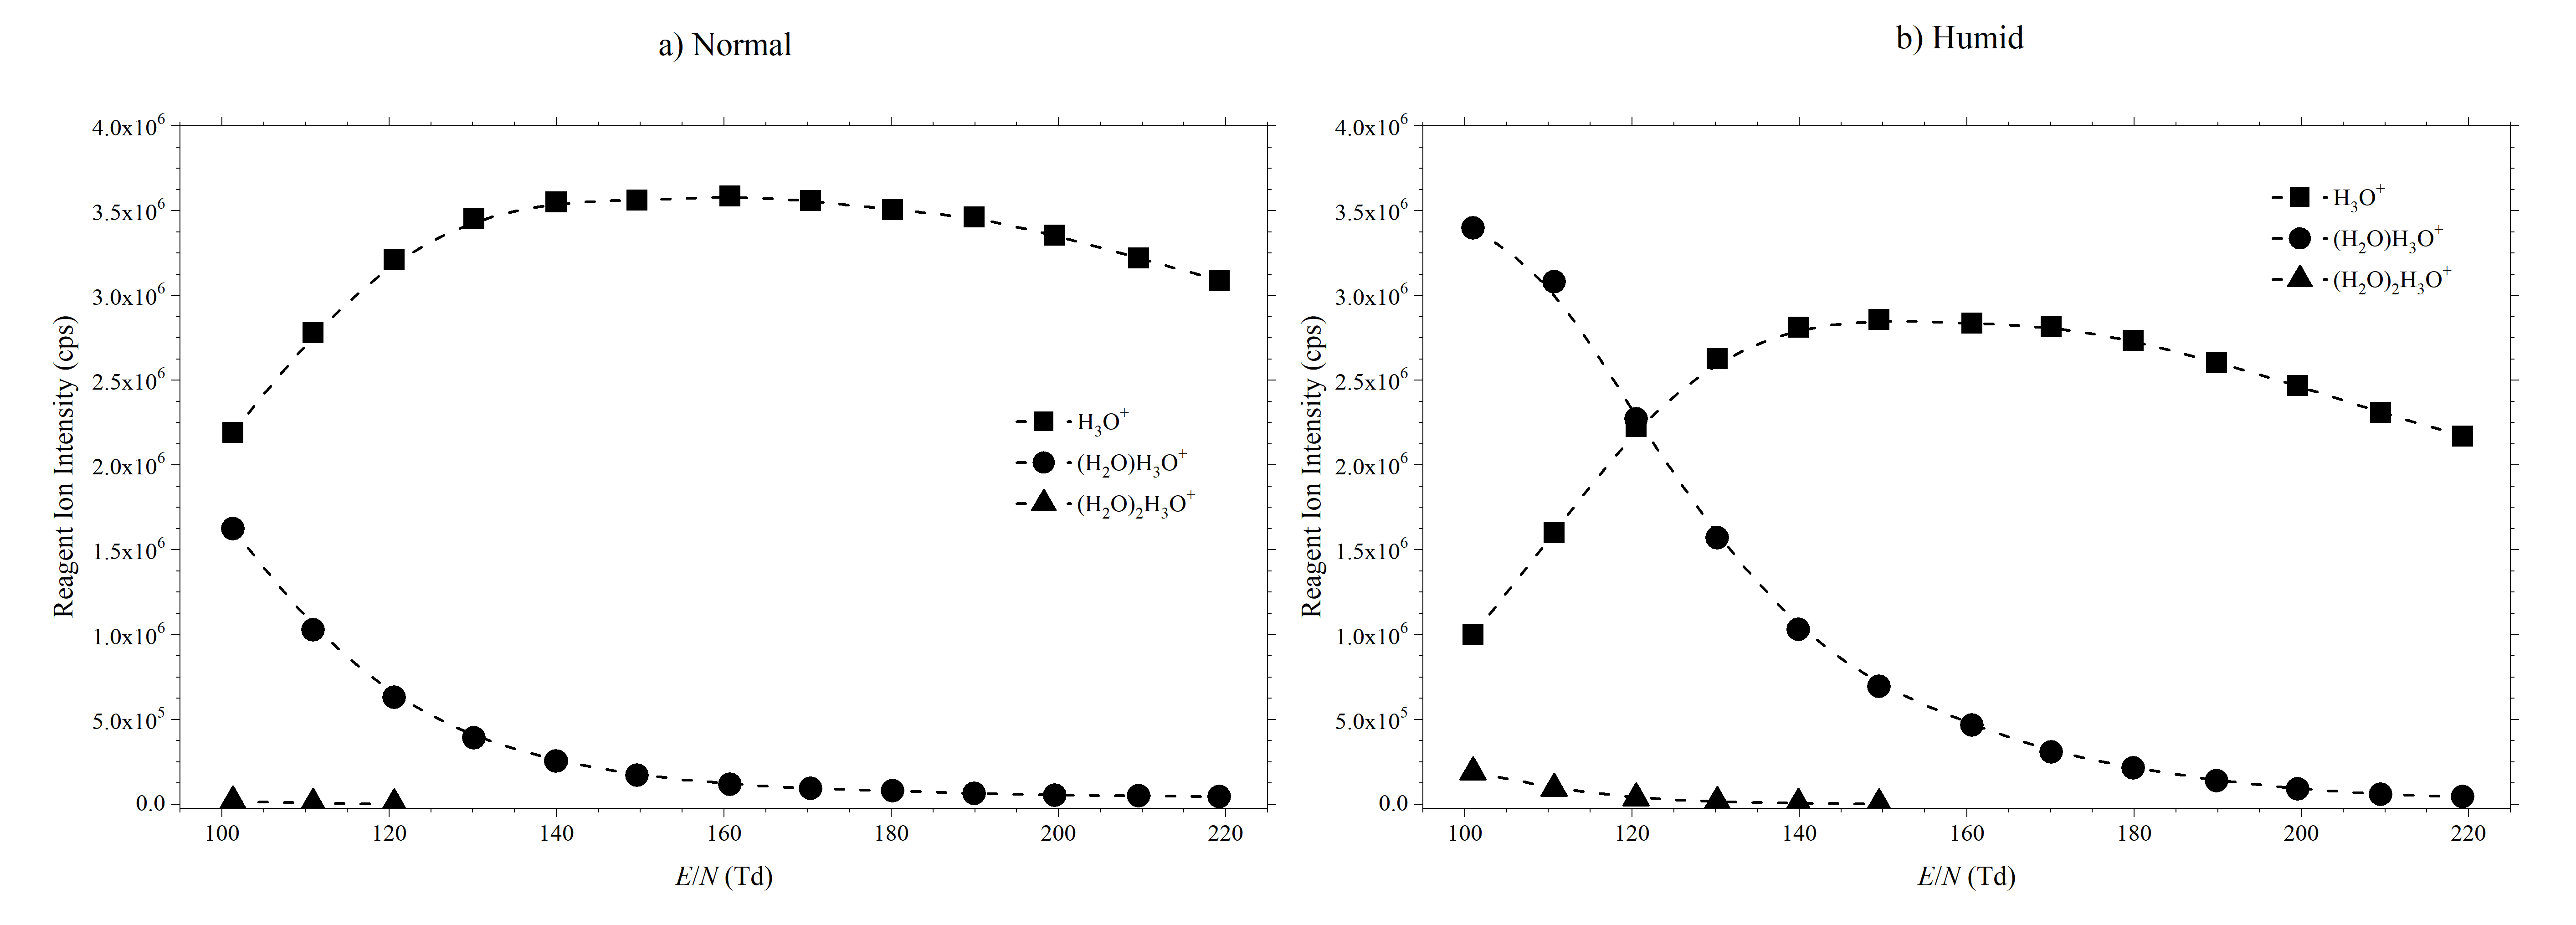
\includegraphics[width=1\textwidth]{pics/ketones/plot_1.png}
\caption{Reagent ion intensities in counts per second (cps) as a function of the reduced electric field for (a) normal (dry buffer gas) and (b) humid (5\% absolute
humidity buffer gas) conditions.}
\label{fig:ke_fig1}
\end{figure}


%These reagent ions are then transported down the drift tube under the influence of the uniform electric field. Analytes are injected into the drift tube through an inlet pipe. Proton transfer from hydronium to the analyte takes place within the drift tube if the proton affinity (PA) of the analyte is higher than that of water (PA(H$_2$O) = 691 kJ mol$^{-1}$). Proton transfer can be non-dissociative and dissociative. However, it should be stressed that fragmentation of the protonated molecule can be a barrierless process and occur spontaneously, or it can be induced by the collision of the reagent ions with analyte and/or charged analyte with the buffer gas.

The drift tube of the PTR-TOF 8000 was kept at 2.3 mbar and 100$^{\circ}$C, being this also the temperature of the inlet line. This values were  the same for all the measurements, giving a constant N, and thus the reduced electric field was solely manipulated by changing the drift voltage in the range from 410 V to 890 V, which corresponds to a \textit{E/N} range from 100 to 220 Td.
To aid in the product ion identification a fastGC was used, which is a modified version of that from \citeauthor{romano2014wine} and \citeauthor{ruzsanyi2013multi} \cite{romano2014wine,ruzsanyi2013multi}.
Details of this device were already given earlier in this thesis (see \autoref{section:fastgc}) and are also available in the literature \cite{malaskova2019compendium}. 
%For all measurements the drift tube was kept at a pressure of 2.3 mbar, with both the inlet system and drift tube being maintained at 100$^{\circ}$C. The collisional energies of the reagent and product ions were controlled by the value of the reduced electric field. For this study we kept the drift tube at constant pressure and temperature (and hence constant N), and changed the drift tube voltage to alter the value of \textit{E/N}. The drift voltage could be changed from 410 V up to a maximum of 890 V. For the applied values of the drift tube pressure and temperature these values correspond to an \textit{E/N} range from 100 Td to 220 Td. 

It is worth clarifying the choice of terms for the operating conditions regarding the humidity in the drift tube. 
Even when the carrier gas is dry N$_2$, some water vapour can diffuse from the ion source into the reactor. Thus, referring to this as “dry” is not totally correct and we will refer to it as the “normal” operating condition. On the other hand, when the carrier gas is not under dry conditions because it has been moisturised in the LCU we will refer to this as “humid” conditions.

%Using a dry buffer gas in the drift tube of a PTR-MS instrument does not mean that it is operated under dry conditions, since some amounts of water vapour diffuse from the hollow cathode. This condition will be denoted as “normal” operating condition later in this paper. When a water saturated buffer gas was used, this is referred in the text as operating the drift tube under “humid” conditions.





%FastGC was used to separate analytes of interest from possible contaminants in the produced standards. The fastGC add-on used in this study is a modification of the setup used by \citeauthor{romano2014wine} \cite{romano2014wine} and \citeauthor{ruzsanyi2013multi} \cite{ruzsanyi2013multi}. Therefore, only the modifications relevant for this study will be provided here. An MXT-1 column (10 m × 0.53 mm, film thickness 0.25 µm, dimethyl polysiloxane phase, Restek, USA) was used. The samples were injected into a 0.5 ml sample loop made of passivated stainless steel. A custom-made valve block consisting of four three-way valves and a needle valve has been replaced by a 10-port passivated valve (VICI AG, Switzerland) and a three-way gas valve made from polyether ether ketone (PEEK) was used. All parts of the inlet system are installed within the oven that houses the drift tube to prevent cold spots. This revised setup enabled constant filling of the sample loop and constant back-flushing of the capillary column with the carrier gas. 8 ml/min and 20 ml/min of 6.0 N$_2$ were used as carrier gas and make-up gas, respectively. A voltage ramp of 0.5 V/s from 10 V up to 80 V was applied raising the temperature of the capillary column from room value up to 240$^{\circ}$C. 












\subsection{Chemicals}
The chemicals used in this study, their purities and their respective providers are:
2-butanone (99.5\%, Honeywell), 
2-pentanone (98\%, Sigma-Aldrich), 
3-pentanone (99\%, Sigma-Aldrich), 
2-hexanone (98\%, Sigma-Aldrich), 
3-hexanone (98\%, Sigma-Aldrich), 
2-heptanone (98.5\%, Honeywell), 
3-heptanone (analytical standard, Sigma-Aldrich), 
4-heptanone (98\%, Sigma-Aldrich), 
3-octanone (99\%, Acros Organics) 
2-nonanone (99\%, Sigma-Aldrich), 
3-nonanone (99\%, Sigma-Aldrich), 
2-decanone (98\%, Sigma-Aldrich), 
3-decanone (97\%, SAFC),
cyclohexanone (99.8\%, Sigma-Aldrich), 
3-methyl-2-pentanone (99\%, Sigma-Aldrich), 
2-methyl-3-pentanone (97\%, Sigma-Aldrich), 
2-methyl-3-hexanone (98\%, Sigma-Aldrich),  
2-methyl-3-heptanone (99\%, Sigma-Aldrich)
and
3-methyl-2-butanone (98.5\%, Honeywell).
No further purification process was applied to these substances.

%The following liquid substances were purchased from Sigma-Aldrich: 2-pentanone (98\%), 3-pentanone (99\%), 2-hexanone (98\%), 3-hexanone (98\%), 3-heptanone (analytical standard), 4-heptanone (98\%), 2-nonanone (99\%), 3-nonanone (99\%), 2-decanone (98\%), cyclohexanone (99.8\%), 3-methyl-2-pentanone (99\%), 2-methyl-3-pentanone (97\%), 2-methyl-3-hexanone (98\%), and 2-methyl-3-heptanone (99\%). 2-butanone (99.5\%), 2-heptanone (98.5\%) and 3-methyl-2-butanone (98.5\%) were purchased from Honeywell. 3-octanone (99\%) and 3-decanone (97\%) were purchased from Acros Organics and SAFC, respectively. These were used with no further purification.





\subsection{Data analysis}
The analysis of the data for this study was done with the “PTR-MS Viewer” (IONICON Analytik GmbH, Austria) software (\autoref{fig:ke_viewer}), which was used to extract the data from the experiment files. 
The multi-peak feature of this software was also useful to separate some isobaric ions, like for example C$_3$H$_3^+$ and the $^{18}$O isotopes of (H$_2$O)H$_3$O$^+$ (i.e. (H$_2\,^{18}$O)H$_3$O$^+$ + (H$_2$O)H$_3\,^{18}$O$^+$), which are both found  at \textit{m/z} 39.
For easier comparison with other instruments, the raw data was not corrected for transmission effects, although it was normalised to 10$^6$ reagent ion counts and the background signals were subtracted. 
Only the ion signal from H$_3$O$^+$ was used to normalise that from  2-butanone (827 kJ mol$^{-1}$), 2-pentanone (833 kJ mol$^{-1}$), 3-pentanone (837 kJ mol$^{-1}$), and 3-methyl-2-butanone (836 kJ mol$^{-1}$) because their proton affinity is higher than that of (H$_2$O)$_2$ (808 kJ mol$^{-1}$). 
For the rest of the ketones, the sum of the counts from H$_3$O$^+$ and (H$_2$O)H$_3$O$^+$ was used to normalise the ion yield.
%However, it is important to note that the product ion distributions of the data acquired with the PTR-TOF 8000 in these experiments can differ from those taken with other equipment and in other conditions.


%The “PTR-MS Viewer” (IONICON Analytik GmbH, Austria) was used to identify peaks in the mass spectra and to extract peak data. Raw peak data, i.e. data not corrected for transmission factors, were normalised to 1 million reagent ions and had any backgrounds subtracted. By using the “raw” data, the product ion distributions we have determined here can be more easily compared with other measurements using different PTR-MS instruments. However, we emphasise that the product ion distributions that have been determined for the selection of ketones chosen for this study have to be taken with some caution if a PTR-TOF 8000 is not being used, and that researchers need to determine product ion distributions for their own instruments and conditions. 



\begin{figure}[t]
\centering
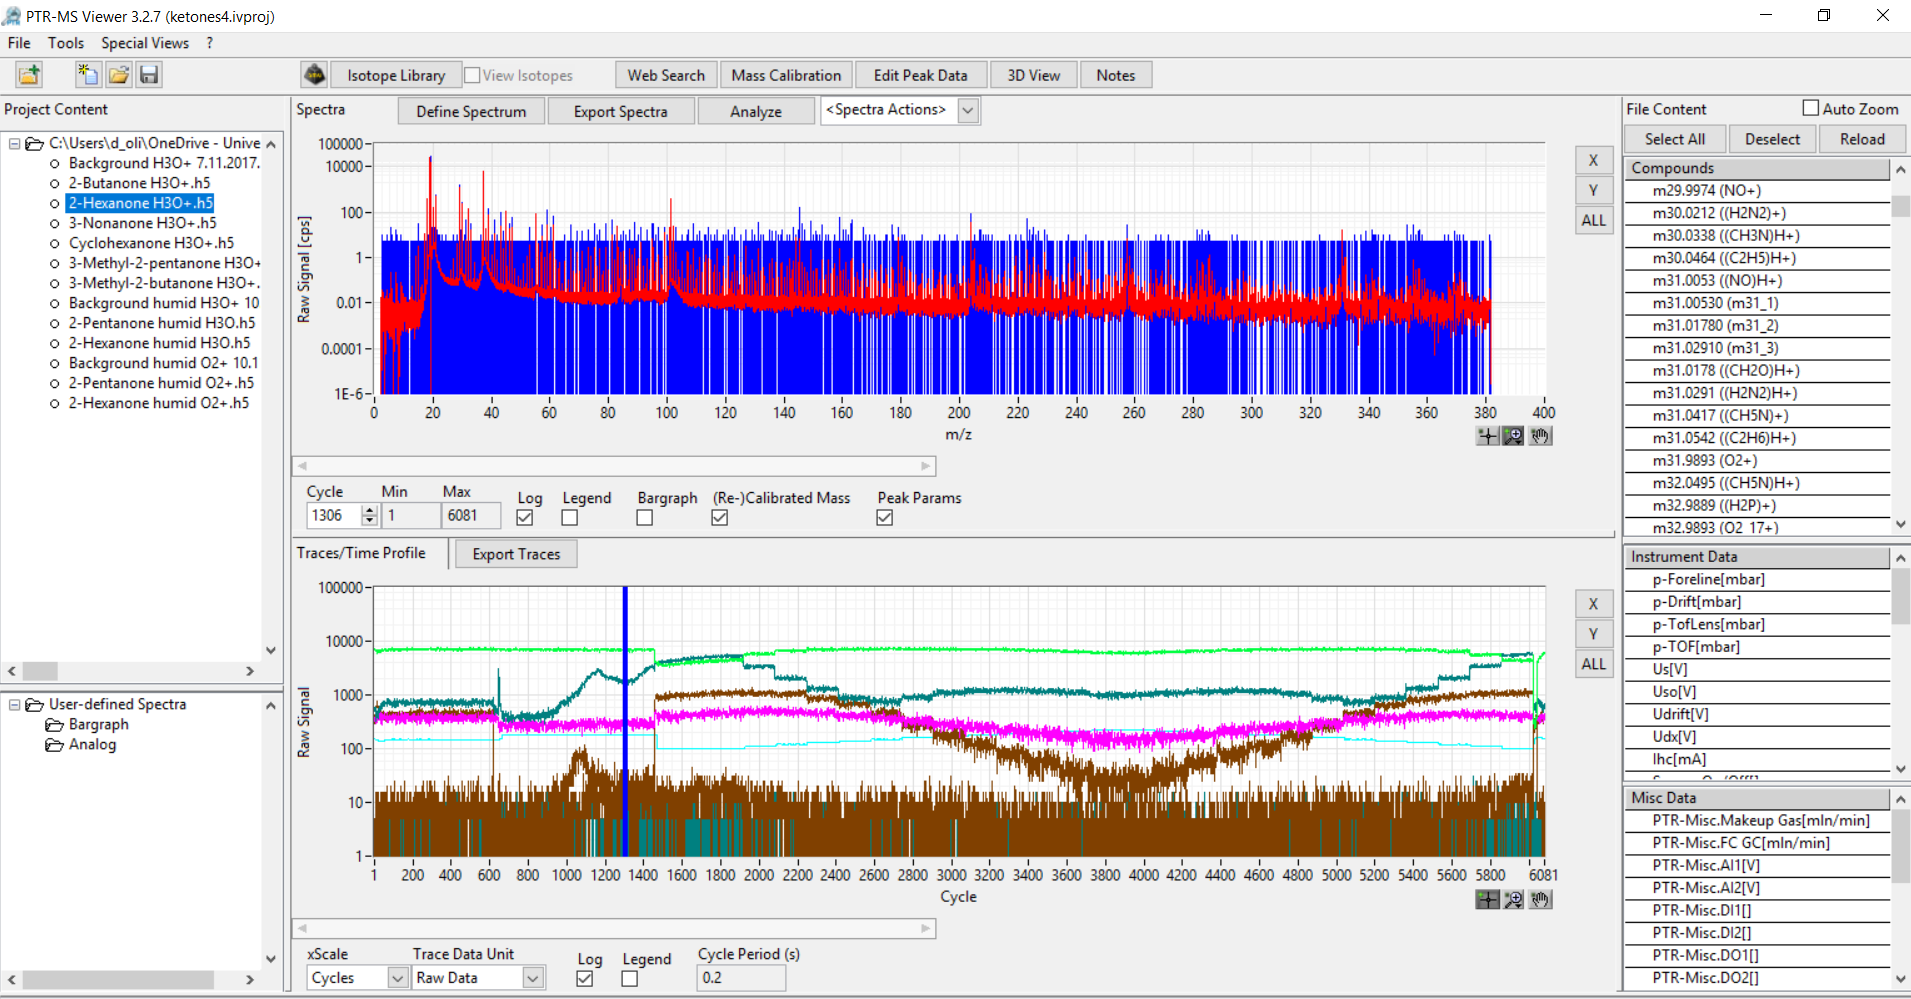
\includegraphics[width=0.8\textwidth]{pics/ptrmsviewer.png}
\caption{Screenshot of the user interface of the PTR-MS Viewer software used for the data analysis in this study.}
\label{fig:ke_viewer}
\end{figure}








\section{Results and Discussion}
The product ion distributions for all the compounds studied in this investigation are shown in \autoref{table:ketones} at 100, 140 and 180 Td for both normal and humid conditions.
These numbers provide a fast picture of the observed product ions for each ketone and show promptly the impacts, if any, of humidity on the distribution of product ions.
The ketones presented in \autoref{table:ketones} (in increasing molecular weight) are thirteen linear, one cyclic and five branched ones.
%\autoref{table:ketones} presents a summary of the product ion distributions (percentages) for all the ketones investigated in this study at three selected reduced electric fields, namely 100 Td, 140 Td and 180 Td under normal and humid conditions. These values give a good representation of all product ions observed and quickly illustrate the effects of humidity on the product ion distributions, if any. The table starts with the thirteen linear chained ketones in order of molecular weight (MW), followed by the one cyclic ketone (cyclohexanone), and finishing with five non-linear ketones, also presented in order of increasing nominal MW, and, for low \textit{E/N} (see \autoref{fig:ke_fig1}), from reactions of H$_3$O$^+$.H$_2$O with those ketones whose proton affinities are greater than that associated with (H$_2$O)$_2$ (808 kJ mol$^{-1}$), i.e. 2-butanone (827 kJ mol$^{-1}$), 2-pentanone (833 kJ mol$^{-1}$), 3-pentanone (837 kJ mol$^{-1}$), and 3-methyl-2-butanone (836 kJ mol$^{-1}$). 
Moreover, \autoref{fig:ke_fig2} graphically presents the product ion distributions as a function of the reduced electric field. 
The product ions considered in this study are those that represent at least 3\% of the total product ion signal at any given \textit{E/N}.
Furthermore, the $^{13}$C peak intensities and the exact \textit{m/z} were used to tentatively assign the product ions to the provided chemical compositions in both \autoref{table:ketones} and \autoref{fig:ke_fig2}.



%The dependence of the product ion branching percentages as a function of \textit{E/N} are shown graphically in \autoref{fig:ke_fig2}. The chemical formulae of the product ions given in \autoref{table:ketones} and \autoref{fig:ke_fig2} have been tentatively identified via the exact \textit{m/z} (to 2 decimal places) and isotope ($^{13}$C) intensities. Only product ions who make a contribution to the branching percentage of at least 3\% at any reduced electric field value are included in the table and figure.

% font needs to be smaller
{\small

\begin{longtable}[c]{lllcccccc}
\caption{Product ions identified and their associated product ion branching ratios (percentages) measured at reduced electric fields of 100, 140, and 180 Td resulting
from the reactions of H$_{3}$O$^+$ with several ketones.}
\label{table:ketones}\\
\hline\textbf{Ketone} & \textbf{Product} & \textbf{Product} & \multicolumn{6}{c}{\textbf{Product Ion Branching Percentages}} \\ \cline{4-9}
\textbf{Molecular Formula} & \textbf{Ion \textit{m/z}} & \textbf{Ion} & \multicolumn{3}{c}{\textbf{Normal \textit{E/N} (Td)}} & \multicolumn{3}{c}{\textbf{Humid \textit{E/N} (Td)}} \\ \cline{4-6} \cline{7-9}
\textbf{Nominal MW} & \textbf{} & \textbf{Formula} & \textbf{100} & \textbf{140} & \textbf{180} & \textbf{100} & \textbf{140} & \textbf{180} \\\hline
\endfirsthead
\hline\textbf{Ketone} & \textbf{Product} & \textbf{Product} & \multicolumn{6}{c}{\textbf{Product Ion Branching Percentages}} \\ \cline{4-9}
\textbf{Molecular Formula} & \textbf{Ion \textit{m/z}} & \textbf{Ion} & \multicolumn{3}{c}{\textbf{Normal \textit{E/N} (Td)}} & \multicolumn{3}{c}{\textbf{Humid \textit{E/N} (Td)}} \\ \cline{4-6} \cline{7-9}
\textbf{Nominal MW} & \textbf{} & \textbf{Formula} & \textbf{100} & \textbf{140} & \textbf{180} & \textbf{100} & \textbf{140} & \textbf{180} \\\hline
\endhead
\textit{(Continued)}
\endfoot
%
\endlastfoot
\multicolumn{9}{c}{Linear ketones} \\ \hline
2-butanone & 73.07 & C$_4$H$_{8}$OH$^+$ & 100 & 99 & 87 & 100 & 100 & 88 \\
C$_4$H$_{8}$O & 55.05 & C$_4$H$_{7}^+$ & 0 & 1 & 10 & 0 & 0 & 10 \\
72 & 39.02 & C$_3$H$_{3}^+$ & 0 & 0 & 3 & 0 & 0 & 2 \\ \hline
2-pentanone & 87.08 & C$_5$H$_{10}$OH$^+$ & 99 & 67 & 20 & 99 & 84 & 29 \\
C$_5$H$_{10}$O & 45.03 & C$_2$H$_{5}$O$^+$ & 1 & 33 & 70 & 1 & 16 & 66 \\
86 & 39.02 & C$_3$H$_{3}^+$ & 0 & 0 & 10 & 0 & 0 & 5 \\ \hline
3-pentanone & 87.08 & C$_5$H$_{10}$OH$^+$ & 98 & 72 & 23 & 99 & 91 & 43 \\
C$_5$H$_{10}$O & 69.07 & C$_5$H$_{9}^+$ & 1 & 4 & 2 & 1 & 4 & 4 \\
86 & 45.03 & C$_2$H$_{5}$O$^+$ & 1 & 20 & 55 & 0 & 4 & 39 \\
 & 41.04 & C$_3$H$_{5}^+$ & 0 & 3 & 5 & 0 & 1 & 5 \\
 & 39.02 & C$_3$H$_{3}^+$ & 0 & 1 & 15 & 0 & 0 & 9 \\ \hline
2-hexanone & 101.1 & C$_6$H$_{12}$OH$^+$ & 100 & 94 & 48 & 100 & 95 & 49 \\
C$_6$H$_{12}$O & 59.05 & C$_3$H$_{7}$O$^+$ & 0 & 1 & 3 & 0 & 1 & 3 \\
100 & 45.03 & C$_2$H$_{5}$O$^+$ & 0 & 5 & 39 & 0 & 4 & 40 \\
 & 39.02 & C$_3$H$_{3}^+$ & 0 & 0 & 10 & 0 & 0 & 8 \\ \hline
3-hexanone & 101.1 & C$_6$H$_{12}$OH$^+$ & 93 & 73 & 31 & 96 & 88 & 44 \\
C$_6$H$_{12}$O & 83.09 & C$_6$H$_{11}^+$ & 1 & 4 & 4 & 1 & 4 & 5 \\
100 & 59.05 & C$_3$H$_{7}$O$^+$ & 3 & 9 & 15 & 3 & 7 & 17 \\
 & 55.05 & C$_4$H$_{7}^+$ & 0 & 3 & 5 & 0 & 0 & 12 \\
 & 45.03 & C$_2$H$_{5}$O$^+$ & 2 & 5 & 15 & 0 & 0 & 0 \\
 & 41.04 & C$_3$H$_{5}^+$ & 0 & 4 & 6 & 0 & 1 & 9 \\
 & 39.02 & C$_3$H$_{3}^+$ & 1 & 1 & 18 & 0 & 0 & 13 \\
 & 31.02 & CH$_{3}$O$^+$ & 0 & 1 & 6 & 0 & 0 & 0 \\ \hline
2-heptanone & 115.11 & C$_7$H$_{14}$OH$^+$ & 94 & 76 & 31 & 96 & 86 & 52 \\
C$_7$H$_{14}$O & 97.1 & C$_7$H$_{13}^+$ & 4 & 10 & 7 & 2 & 7 & 9 \\
114 & 59.05 & C$_3$H$_{7}$O$^+$ & 1 & 2 & 4 & 2 & 3 & 6 \\
 & 55.05 & C$_4$H$_{7}^+$ & 0 & 9 & 14 & 0 & 4 & 20 \\
 & 45.03 & C$_2$H$_{5}$O$^+$ & 1 & 3 & 15 & 0 & 0 & 0 \\
 & 39.02 & C$_3$H$_{3}^+$ & 0 & 0 & 29 & 0 & 0 & 13 \\ \hline
3-heptanone & 115.11 & C$_7$H$_{14}$OH$^+$ & 98 & 89 & 35 & 99 & 95 & 57 \\
C$_7$H$_{14}$O & 97.1 & C$_7$H$_{13}^+$ & 2 & 5 & 4 & 1 & 4 & 5 \\
114 & 59.05 & C$_3$H$_{7}$O$^+$ & 0 & 0 & 0 & 0 & 1 & 7 \\
 & 55.05 & C$_4$H$_{7}^+$ & 0 & 4 & 8 & 0 & 0 & 12 \\
 & 41.04 & C$_3$H$_{5}^+$ & 0 & 1 & 7 & 0 & 0 & 3 \\
 & 39.02 & C$_3$H$_{3}^+$ & 0 & 0 & 27 & 0 & 0 & 16 \\
 & 31.02 & CH$_{3}$O$^+$ & 0 & 1 & 19 & 0 & 0 & 0 \\ \hline
4-heptanone & 115.11 & C$_7$H$_{14}$OH$^+$ & 98 & 90 & 52 & 99 & 95 & 70 \\
C$_7$H$_{14}$O & 73.07 & C$_4$H$_{9}$O$^+$ & 0 & 1 & 2 & 0 & 0 & 0 \\
114 & 59.05 & C$_3$H$_{7}$O$^+$ & 1 & 2 & 6 & 1 & 1 & 4 \\
 & 55.05 & C$_4$H$_{7}^+$ & 0 & 6 & 15 & 0 & 4 & 16 \\
 & 53.04 & C$_4$H$_{5}^+$ & 0 & 0 & 5 & 0 & 0 & 3 \\
 & 39.02 & C$_3$H$_{3}^+$ & 1 & 1 & 20 & 0 & 0 & 7 \\ \hline
3-octanone & 129.13 & C$_8$H$_{16}$OH$^+$ & 99 & 96 & 46 & 100 & 98 & 73 \\
C$_8$H$_{16}$O & 69.07 & C$_5$H$_{9}^+$ & 0 & 3 & 5 & 0 & 1 & 6 \\
128 & 59.05 & C$_3$H$_{7}$O$^+$ & 1 & 1 & 3 & 0 & 1 & 4 \\
 & 41.04 & C$_3$H$_{5}^+$ & 0 & 0 & 11 & 0 & 0 & 10 \\
 & 39.02 & C$_3$H$_{3}^+$ & 0 & 0 & 35 & 0 & 0 & 7 \\ \hline
2-nonanone & 143.14 & C$_9$H$_{18}$OH$^+$ & 100 & 93 & 34 & 100 & 97 & 62 \\
C$_9$H$_{18}$O & 83.09 & C$_6$H$_{11}^+$ & 0 & 0 & 0 & 0 & 1 & 4 \\
142 & 69.07 & C$_5$H$_{9}^+$ & 0 & 4 & 4 & 0 & 2 & 6 \\
 & 55.05 & C$_4$H$_{7}^+$ & 0 & 1 & 4 & 0 & 0 & 7 \\
 & 41.04 & C$_3$H$_{5}^+$ & 0 & 1 & 10 & 0 & 0 & 10 \\
 & 39.02 & C$_3$H$_{3}^+$ & 0 & 1 & 48 & 0 & 0 & 11 \\ \hline
3-nonanone & 143.14 & C$_9$H$_{18}$OH$^+$ & 100 & 87 & 48 & 100 & 100 & 79 \\
C$_9$H$_{18}$O & 55.05 & C$_4$H$_{7}^+$ & 0 & 4 & 6 & 0 & 0 & 5 \\
142 & 41.04 & C$_3$H$_{5}^+$ & 0 & 8 & 11 & 0 & 0 & 6 \\
 & 39.02 & C$_3$H$_{3}^+$ & 0 & 1 & 35 & 0 & 0 & 10 \\ \hline
2-decanone & 157.16 & C$_{10}$H$_{20}$OH$^+$ & 100 & 94 & 48 & 100 & 99 & 81 \\
C$_{10}$H$_{20}$O & 83.09 & C$_6$H$_{11}^+$ & 0 & 2 & 3 & 0 & 1 & 6 \\
156 & 55.05 & C$_4$H$_{7}^+$ & 0 & 3 & 13 & 0 & 0 & 13 \\
 & 39.02 & C$_3$H$_{3}^+$ & 0 & 1 & 36 & 0 & 0 & 0 \\ \hline
3-decanone & 157.16 & C$_{10}$H$_{20}$OH$^+$ & 99 & 95 & 48 & 100 & 100 & 86 \\
C$_{10}$H$_{20}$O & 55.05 & C$_4$H$_{7}^+$ & 1 & 4 & 10 & 0 & 0 & 7 \\
156 & 39.02 & C$_3$H$_{3}^+$ & 0 & 1 & 42 & 0 & 0 & 7 \\ \hline
\multicolumn{9}{c}{Cyclic ketone} \\ \hline
cyclohexanone & 99.08 & C$_6$H$_{10}$OH$^+$ & 99 & 88 & 30 & 99 & 93 & 40 \\
C$_6$H$_{10}$O & 81.07 & C$_6$H$_{9}^+$ & 1 & 12 & 65 & 1 & 7 & 56 \\
98 & 79.05 & C$_6$H$_{7}^+$ & 0 & 0 & 5 & 0 & 0 & 3 \\
 & 39.02 & C$_3$H$_{3}^+$ & 0 & 0 & 0 & 0 & 0 & 1 \\ \hline
\multicolumn{9}{c}{Branched ketones} \\ \hline
3-methyl-2-butanone & 87.08 & C$_5$H$_{10}$OH$^+$ & 100 & 98 & 63 & 99 & 96 & 66 \\
C$_5$H$_{10}$O & 69.07 & C$_5$H$_{9}^+$ & 0 & 2 & 5 & 1 & 3 & 7 \\
86 & 45.03 & C$_2$H$_{5}$O$^+$ & 0 & 0 & 8 & 0 & 0 & 8 \\
 & 41.04 & C$_3$H$_{5}^+$ & 0 & 0 & 4 & 0 & 1 & 8 \\
 & 39.02 & C$_3$H$_{3}^+$ & 0 & 0 & 20 & 0 & 0 & 11 \\ \hline
3-methyl-2-pentanone & 101.1 & C$_6$H$_{12}$OH$^+$ & 100 & 70 & 23 & 100 & 73 & 22 \\
C$_6$H$_{12}$O & 59.05 & C$_3$H$_{7}$O$^+$ & 0 & 11 & 28 & 0 & 7 & 26 \\
100 & 57.07 & C$_4$H$_{9}^+$ & 0 & 4 & 3 & 0 & 5 & 4 \\
 & 45.03 & C$_2$H$_{5}$O$^+$ & 0 & 15 & 39 & 0 & 15 & 40 \\
 & 39.02 & C$_3$H$_{3}^+$ & 0 & 0 & 7 & 0 & 0 & 8 \\ \hline
2-methyl-3-pentanone & 101.1 & C$_6$H$_{12}$OH$^+$ & 98 & 61 & 17 & 95 & 74 & 24 \\
C$_6$H$_{12}$O & 59.05 & C$_3$H$_{7}$O$^+$ & 1 & 15 & 29 & 3 & 9 & 29 \\
100 & 57.07 & C$_4$H$_{9}^+$ & 0 & 4 & 2 & 0 & 3 & 3 \\
 & 45.03 & C$_2$H$_{5}$O$^+$ & 1 & 20 & 41 & 2 & 13 & 40 \\
 & 39.02 & C$_3$H$_{3}^+$ & 0 & 0 & 11 & 0 & 1 & 4 \\ \hline
2-methyl-3-hexanone & 115.11 & C$_7$H$_{14}$OH$^+$ & 95 & 66 & 24 & 96 & 72 & 24 \\
C$_7$H$_{14}$O & 97.1 & C$_7$H$_{13}^+$ & 5 & 14 & 8 & 4 & 10 & 7 \\
114 & 59.05 & C$_3$H$_{7}$O$^+$ & 0 & 8 & 17 & 0 & 4 & 17 \\
 & 55.05 & C$_4$H$_{7}^+$ & 0 & 4 & 5 & 0 & 2 & 7 \\
 & 45.03 & C$_2$H$_{5}$O$^+$ & 0 & 5 & 17 & 0 & 11 & 27 \\
 & 41.04 & C$_3$H$_{5}^+$ & 0 & 3 & 7 & 0 & 1 & 6 \\
 & 39.02 & C$_3$H$_{3}^+$ & 0 & 0 & 22 & 0 & 0 & 12 \\ \hline
2-methyl-3-heptanone & 129.13 & C$_8$H$_{16}$OH$^+$ & 96 & 76 & 26 & 97 & 81 & 28 \\
C$_8$H$_{16}$O & 111.12 & C$_8$H$_{15}^+$ & 3 & 5 & 3 & 2 & 5 & 3 \\
128 & 69.07 & C$_5$H$_{9}^+$ & 0 & 8 & 5 & 0 & 4 & 5 \\
 & 59.05 & C$_3$H$_{7}$O$^+$ & 0 & 0 & 0 & 0 & 3 & 14 \\
 & 45.03 & C$_2$H$_{5}$O$^+$ & 0 & 2 & 8 & 0 & 3 & 10 \\
 & 43.05 & C$_3$H$_{7}^+$ & 1 & 2 & 2 & 1 & 2 & 3 \\
 & 41.04 & C$_3$H$_{5}^+$ & 0 & 6 & 15 & 0 & 2 & 15 \\
 & 39.02 & C$_3$H$_{3}^+$ & 0 & 1 & 41 & 0 & 0 & 22\\ \hline
\end{longtable}
}%closing small font


\captionsetup{list=no} % this removes the several continued captions from the figures list
\begin{figure}%[h]\ContinuedFloat
\centering
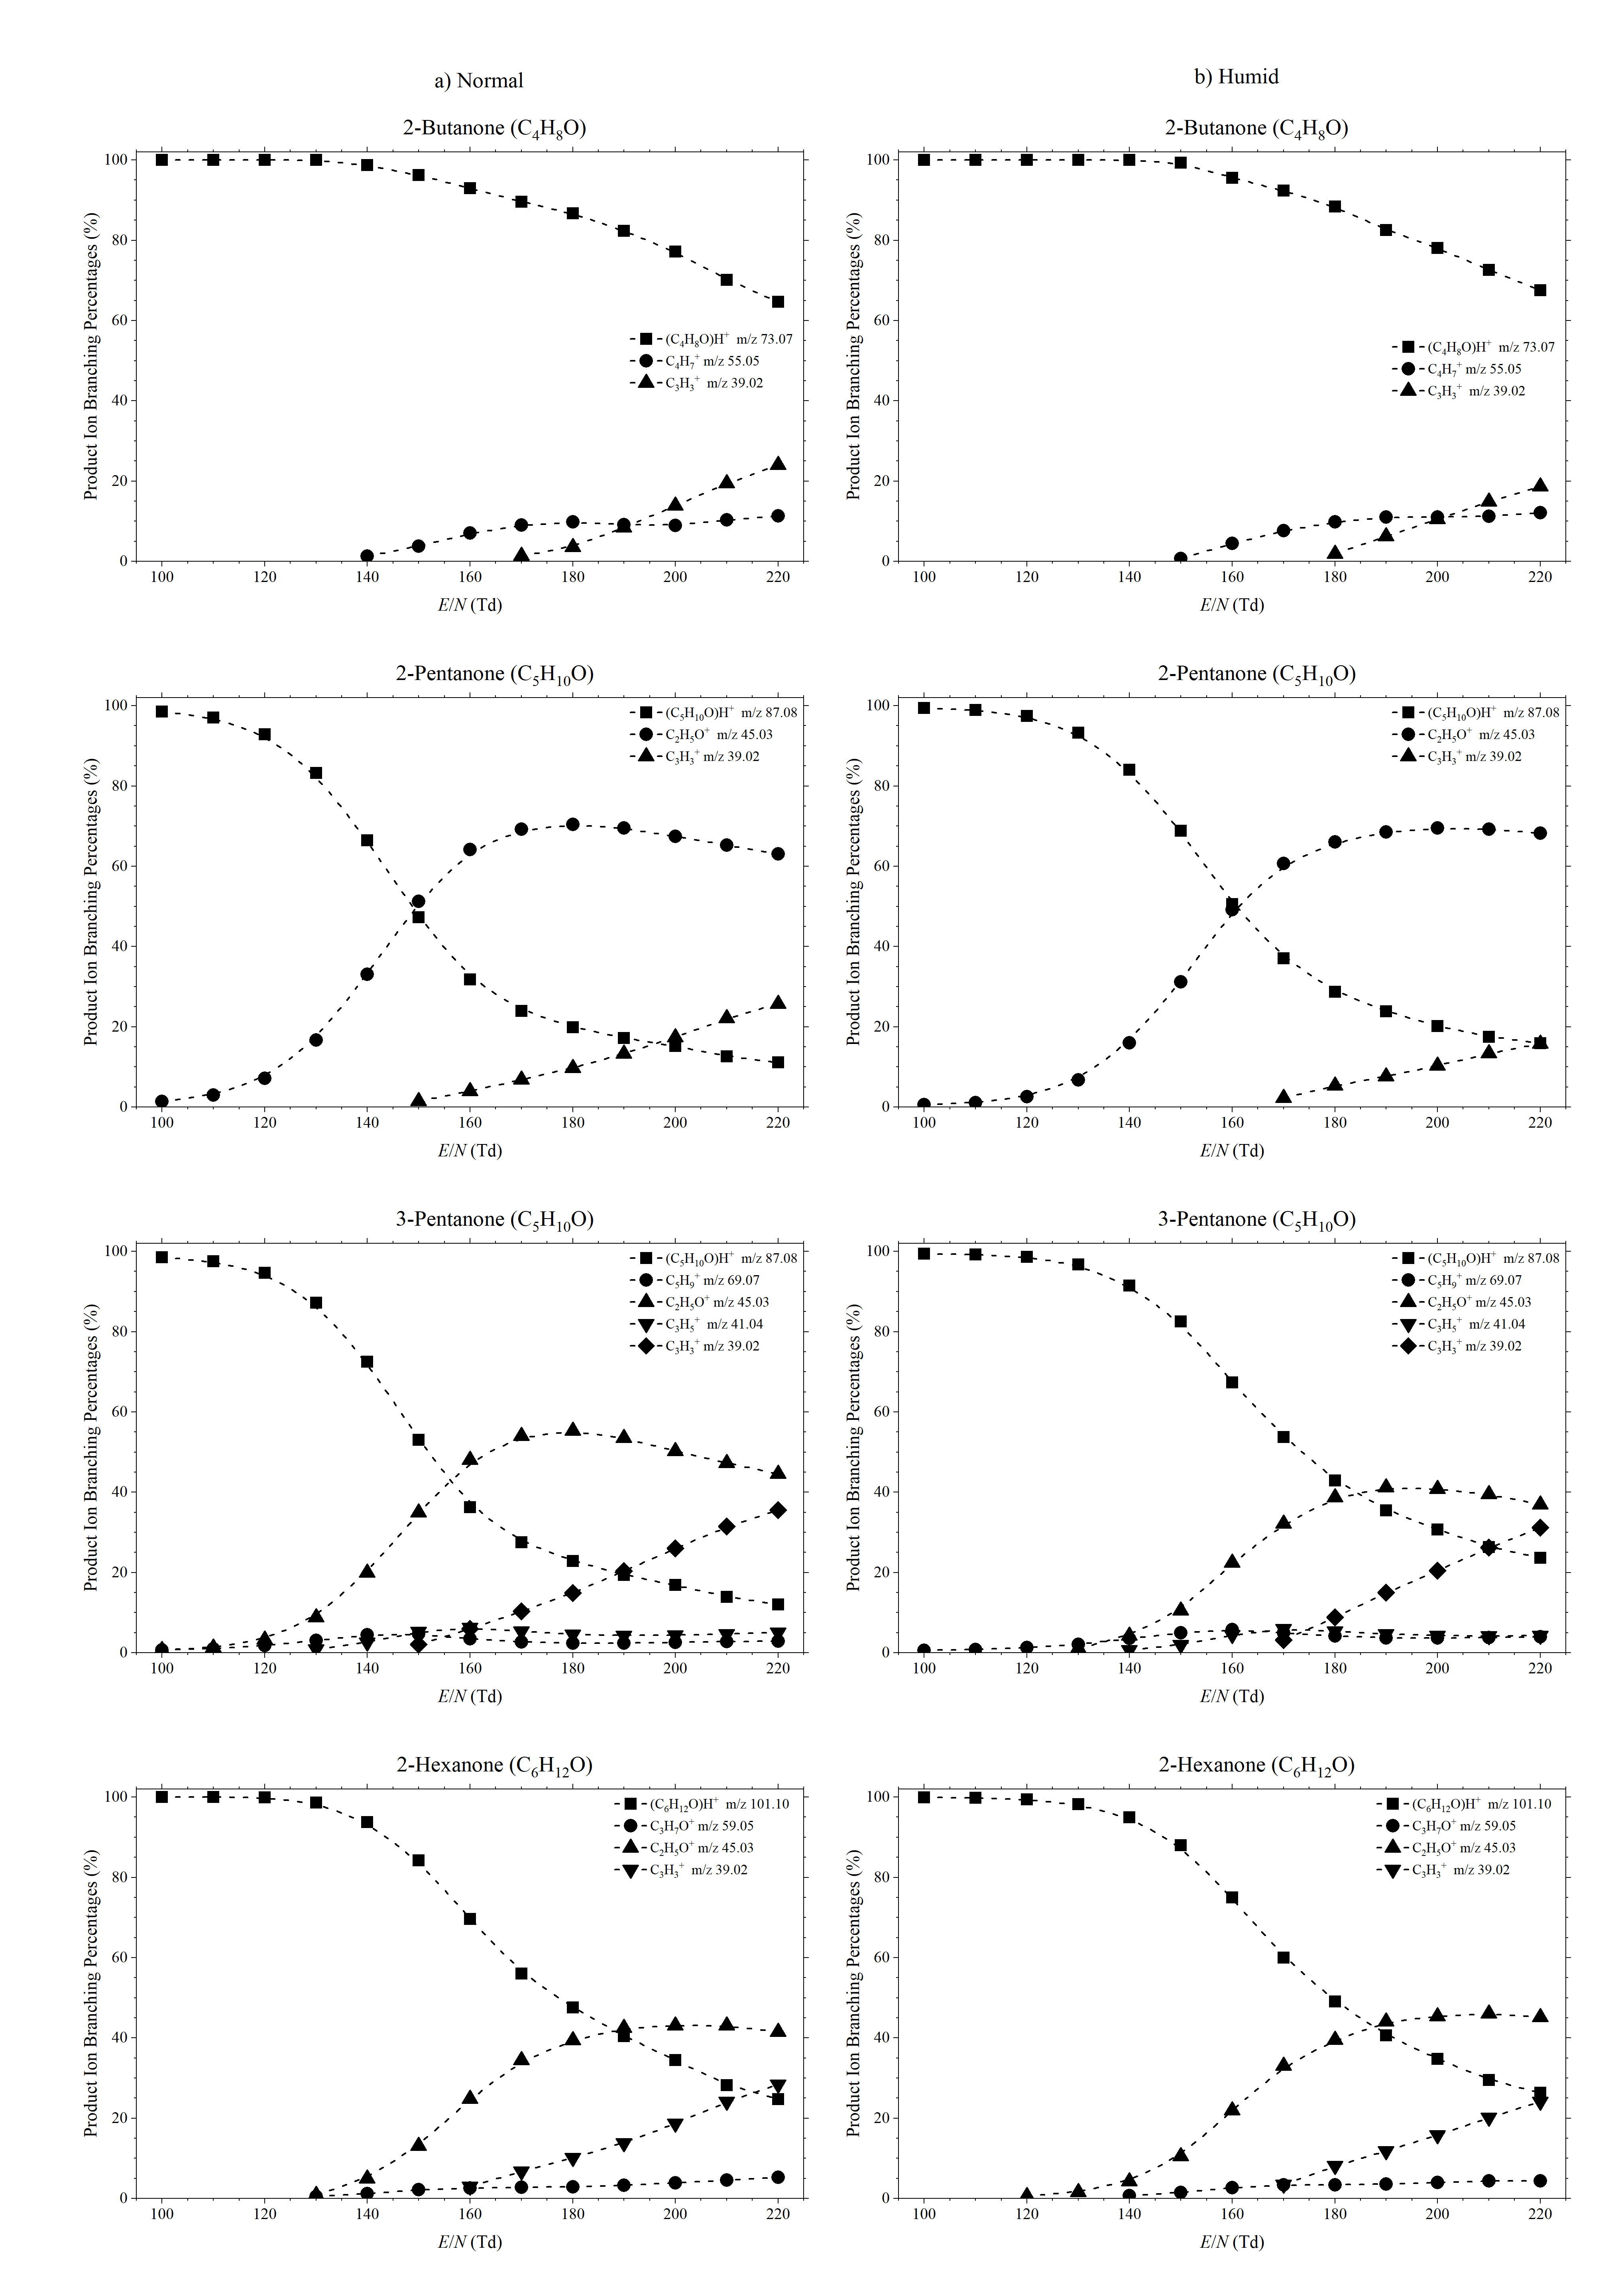
\includegraphics[width=1\textwidth]{pics/ketones/plot_2.png}
\caption{\textit{Continued}}
\end{figure}
\begin{figure}\ContinuedFloat
\centering
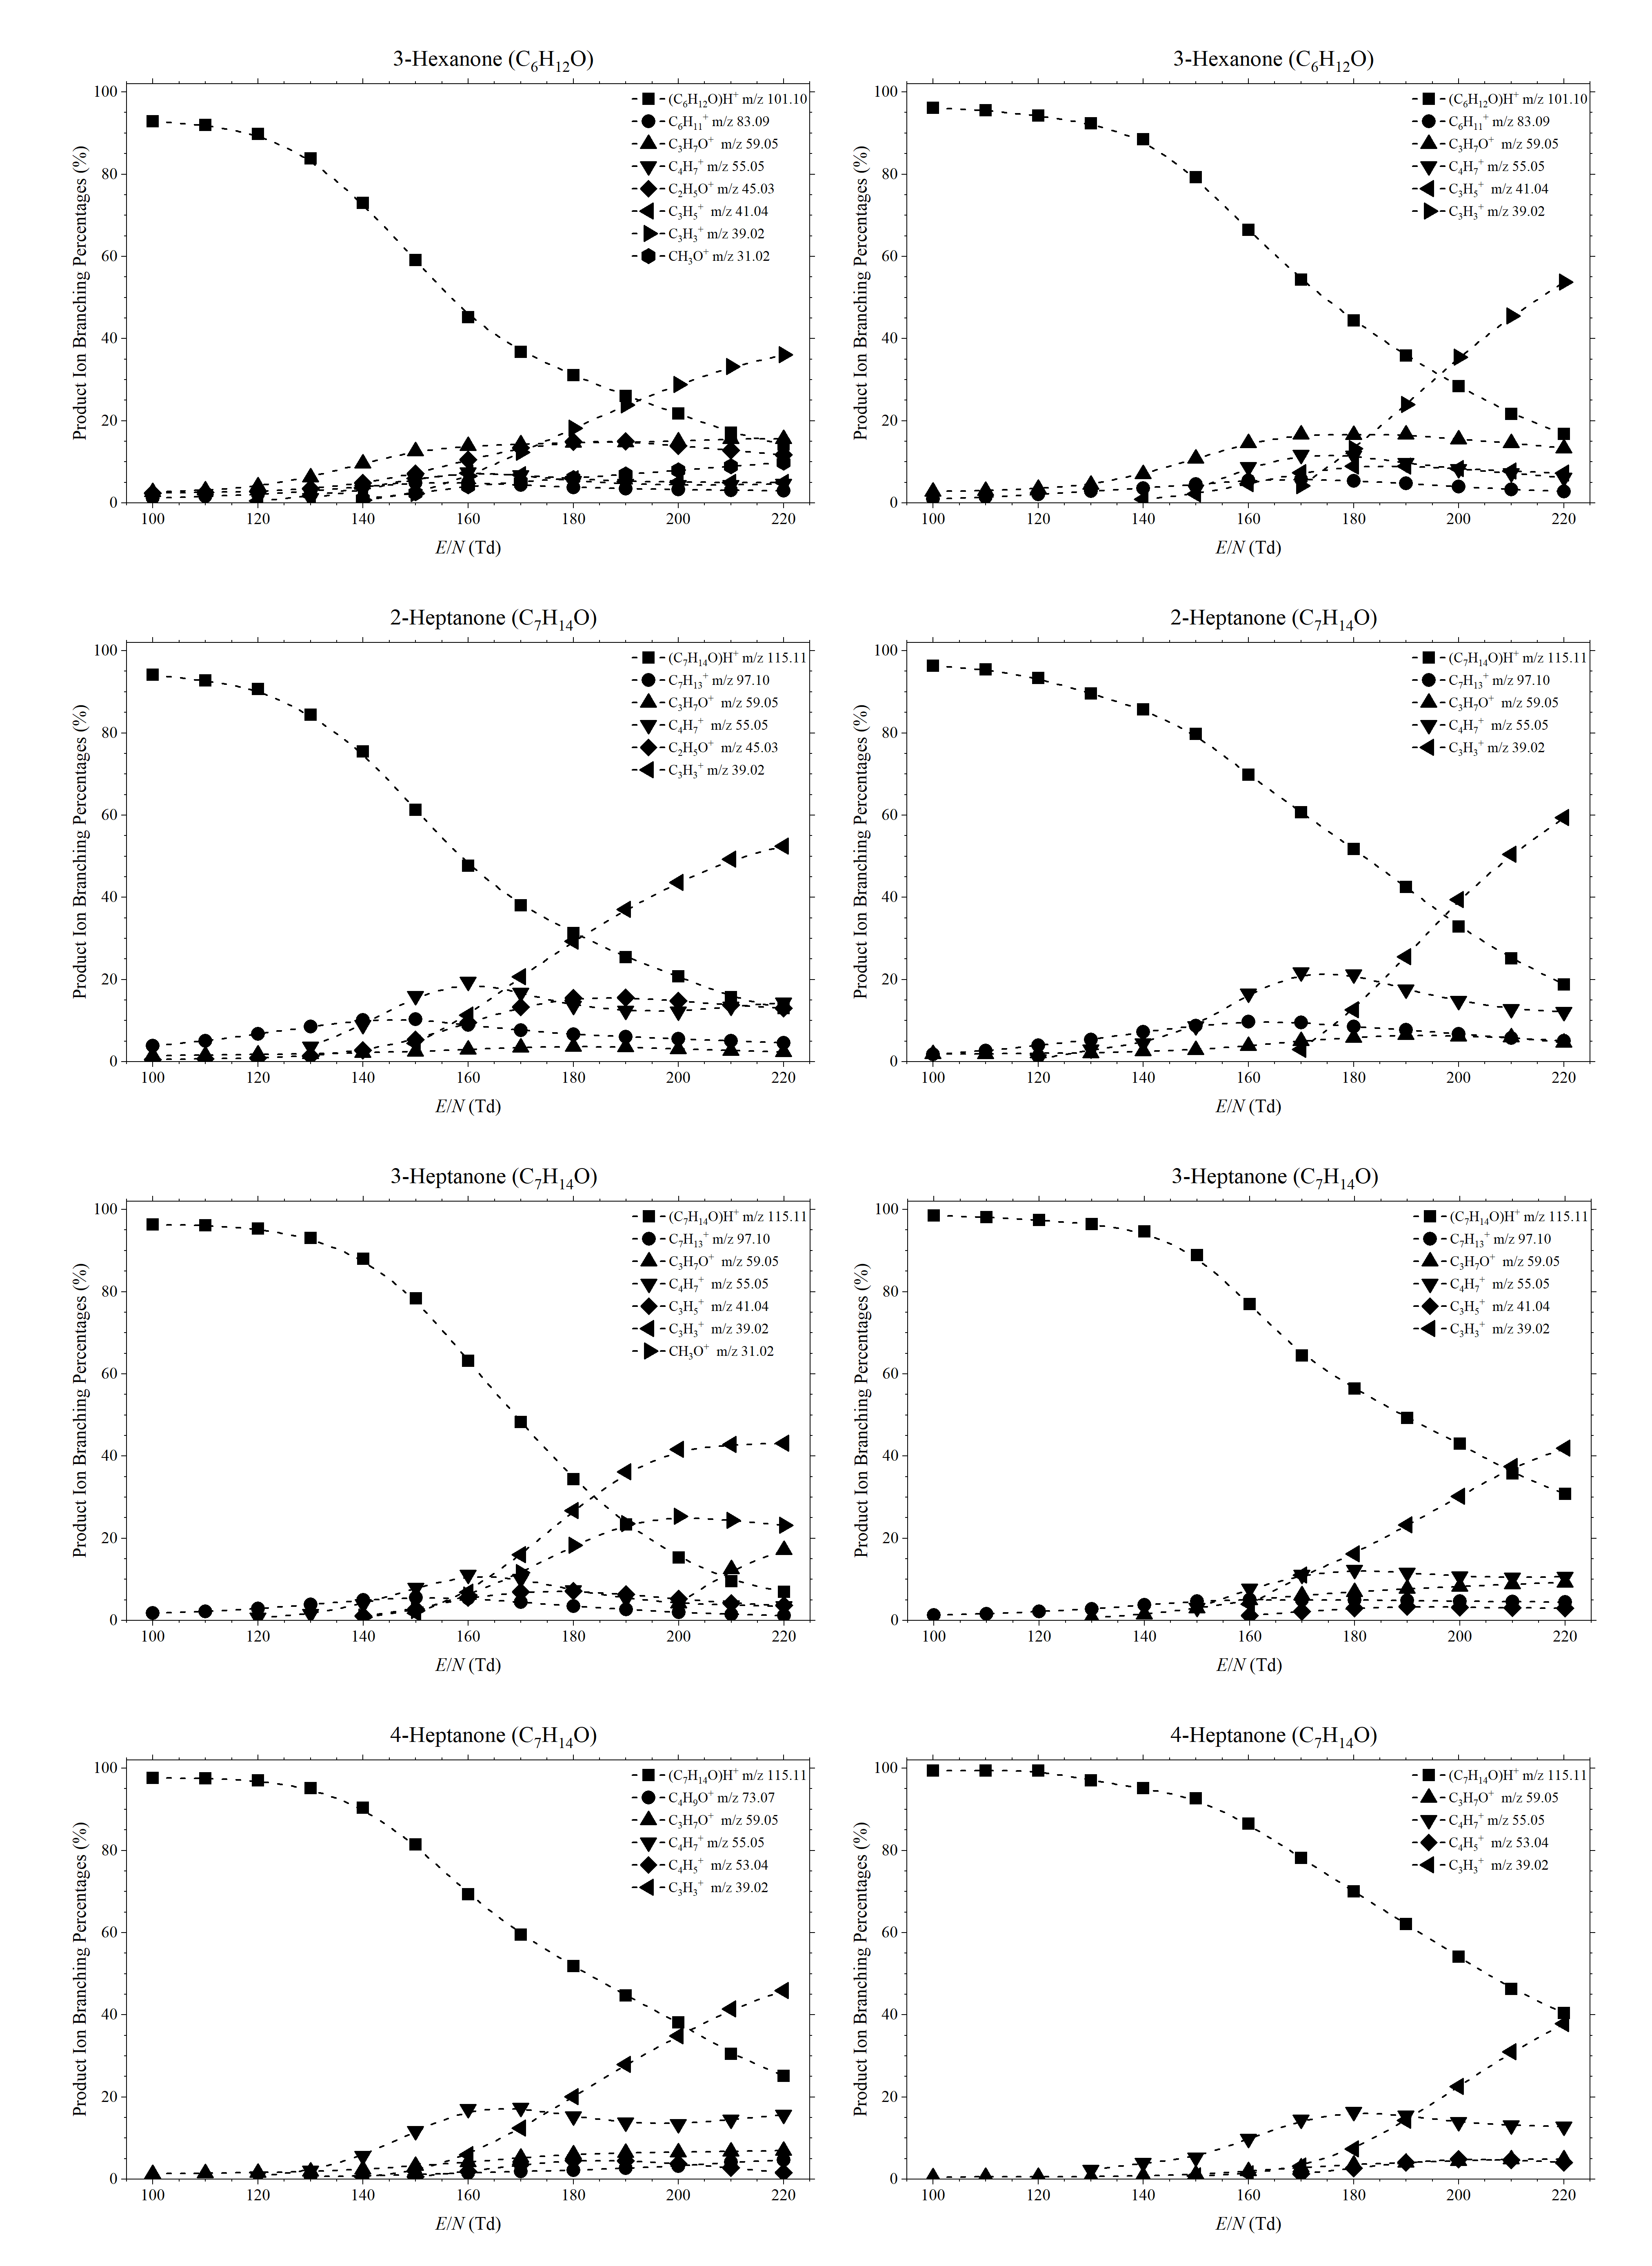
\includegraphics[width=1\textwidth]{pics/ketones/plot_3.png}
\caption{\textit{Continued}}
\end{figure}
\begin{figure}\ContinuedFloat
\centering
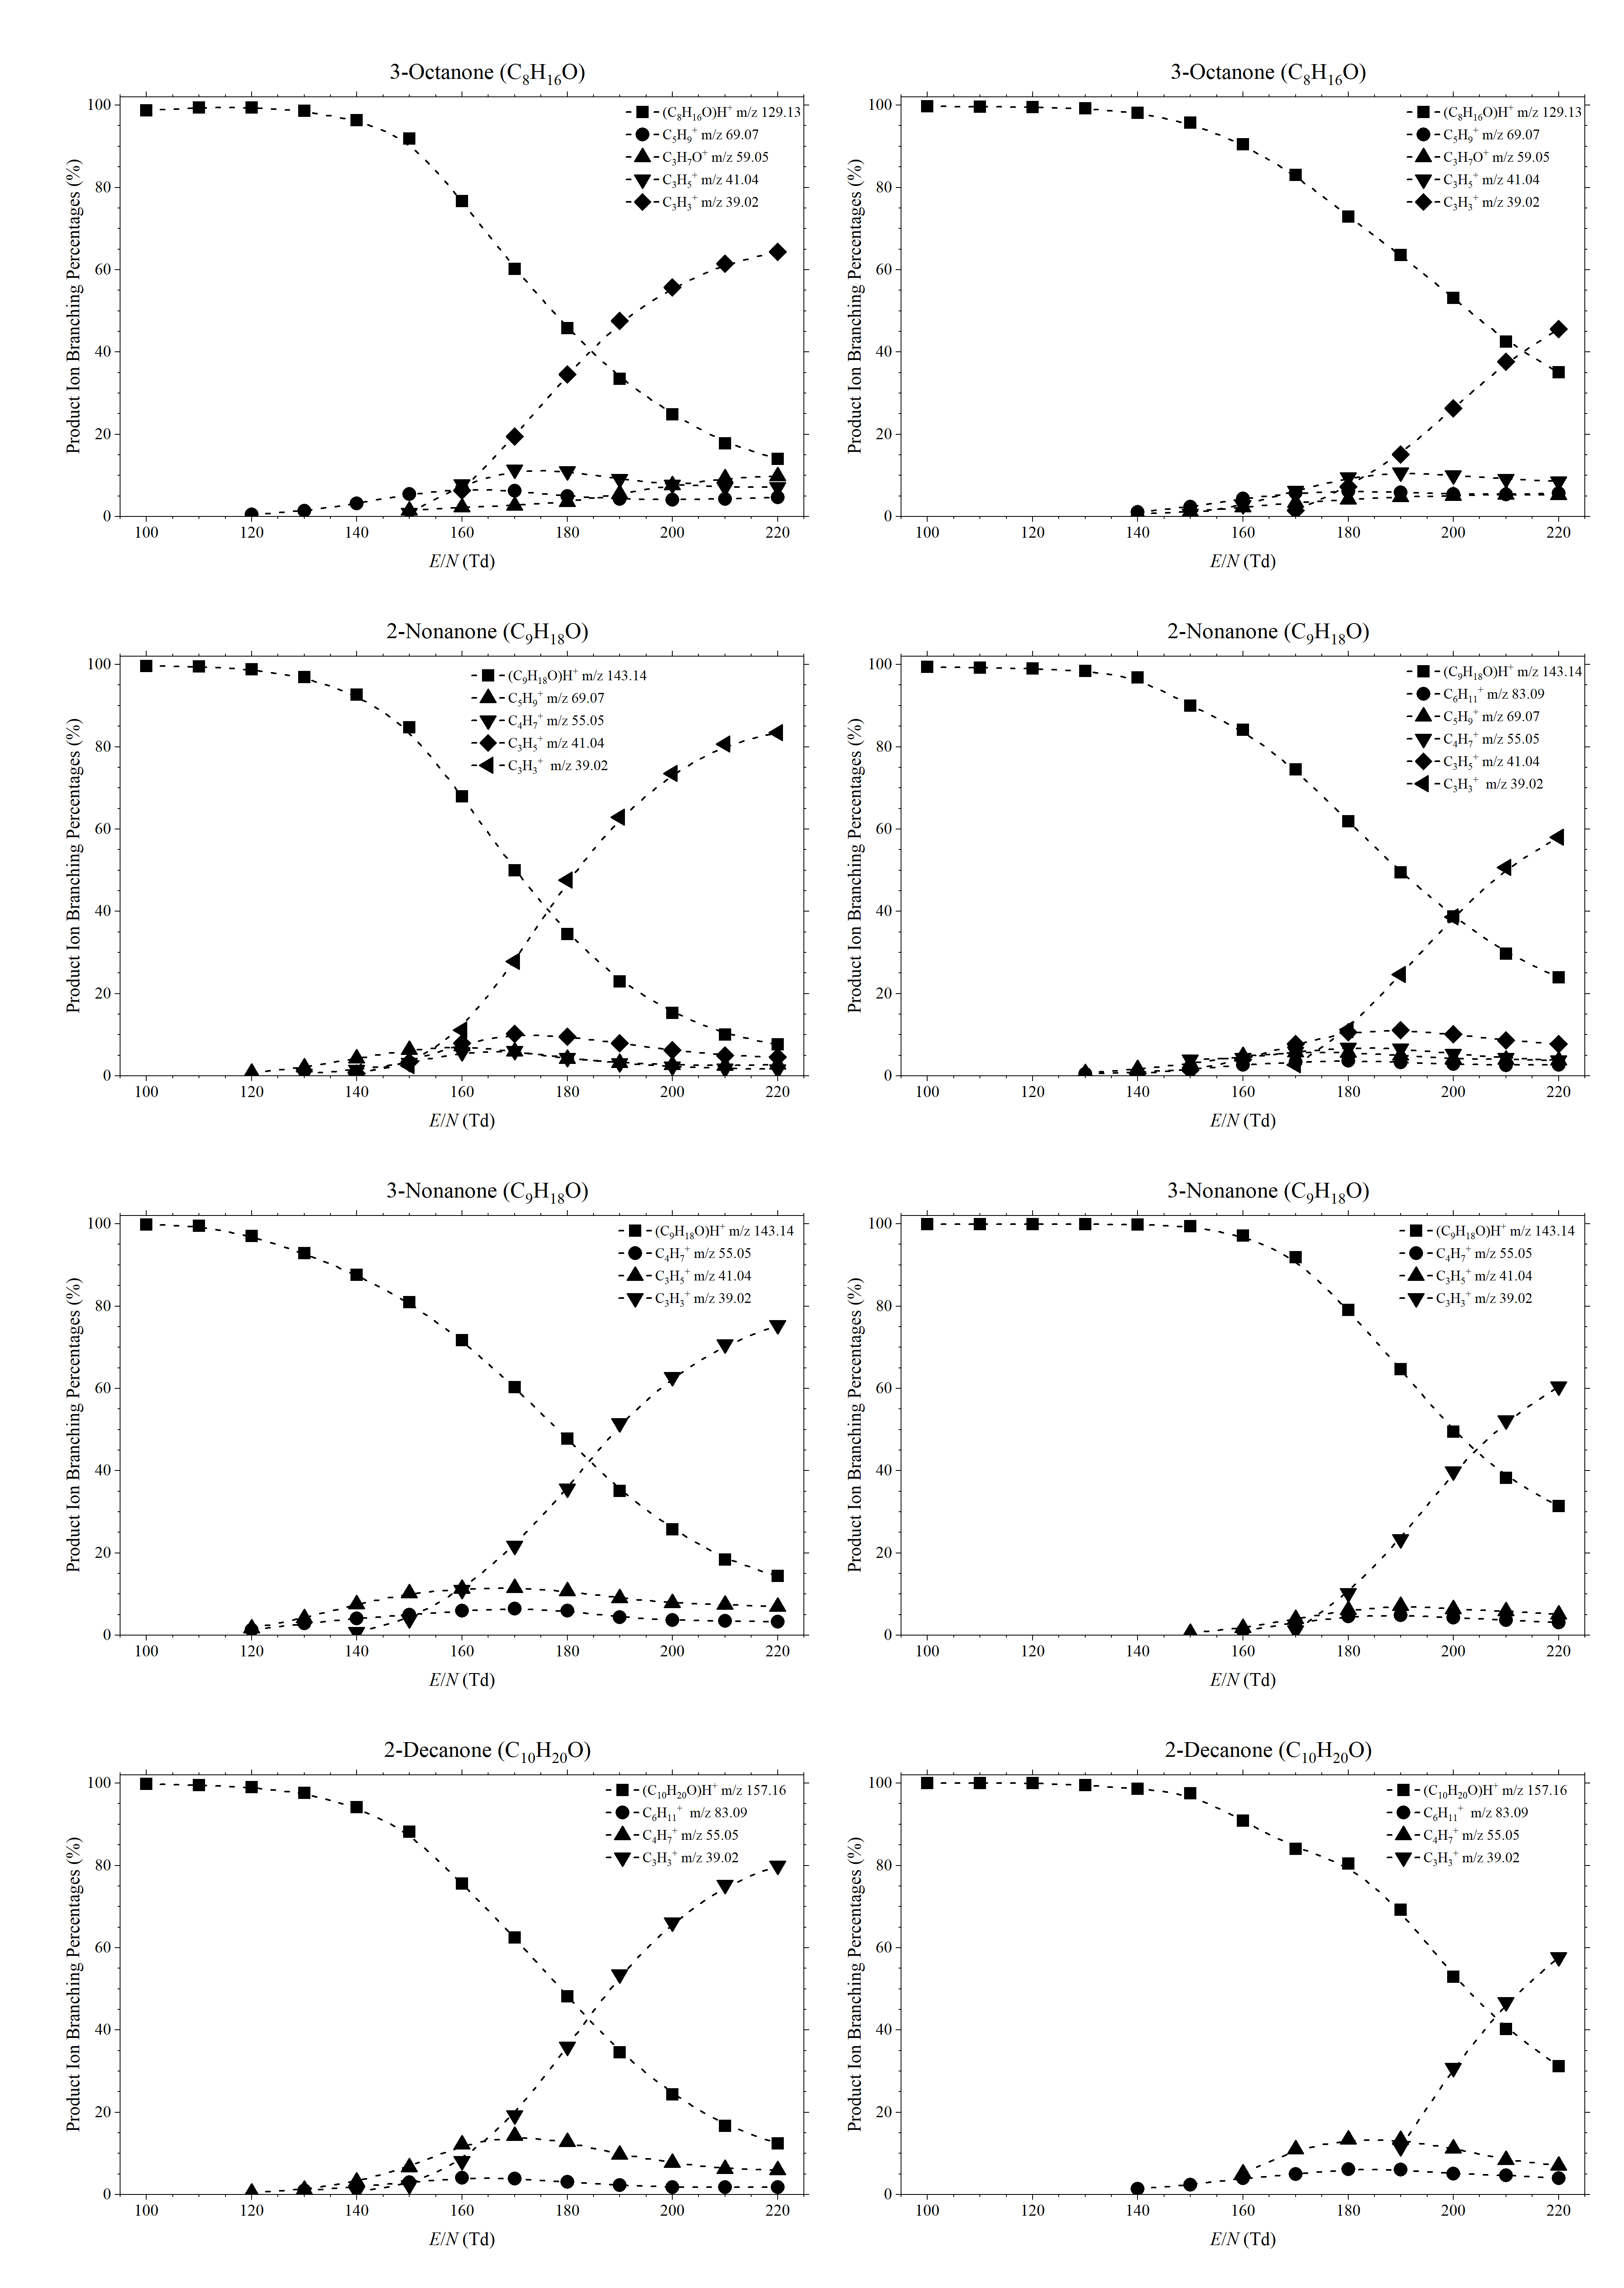
\includegraphics[width=1\textwidth]{pics/ketones/plot_4.png}
\caption{\textit{Continued}}
\end{figure}
\begin{figure}\ContinuedFloat
\centering
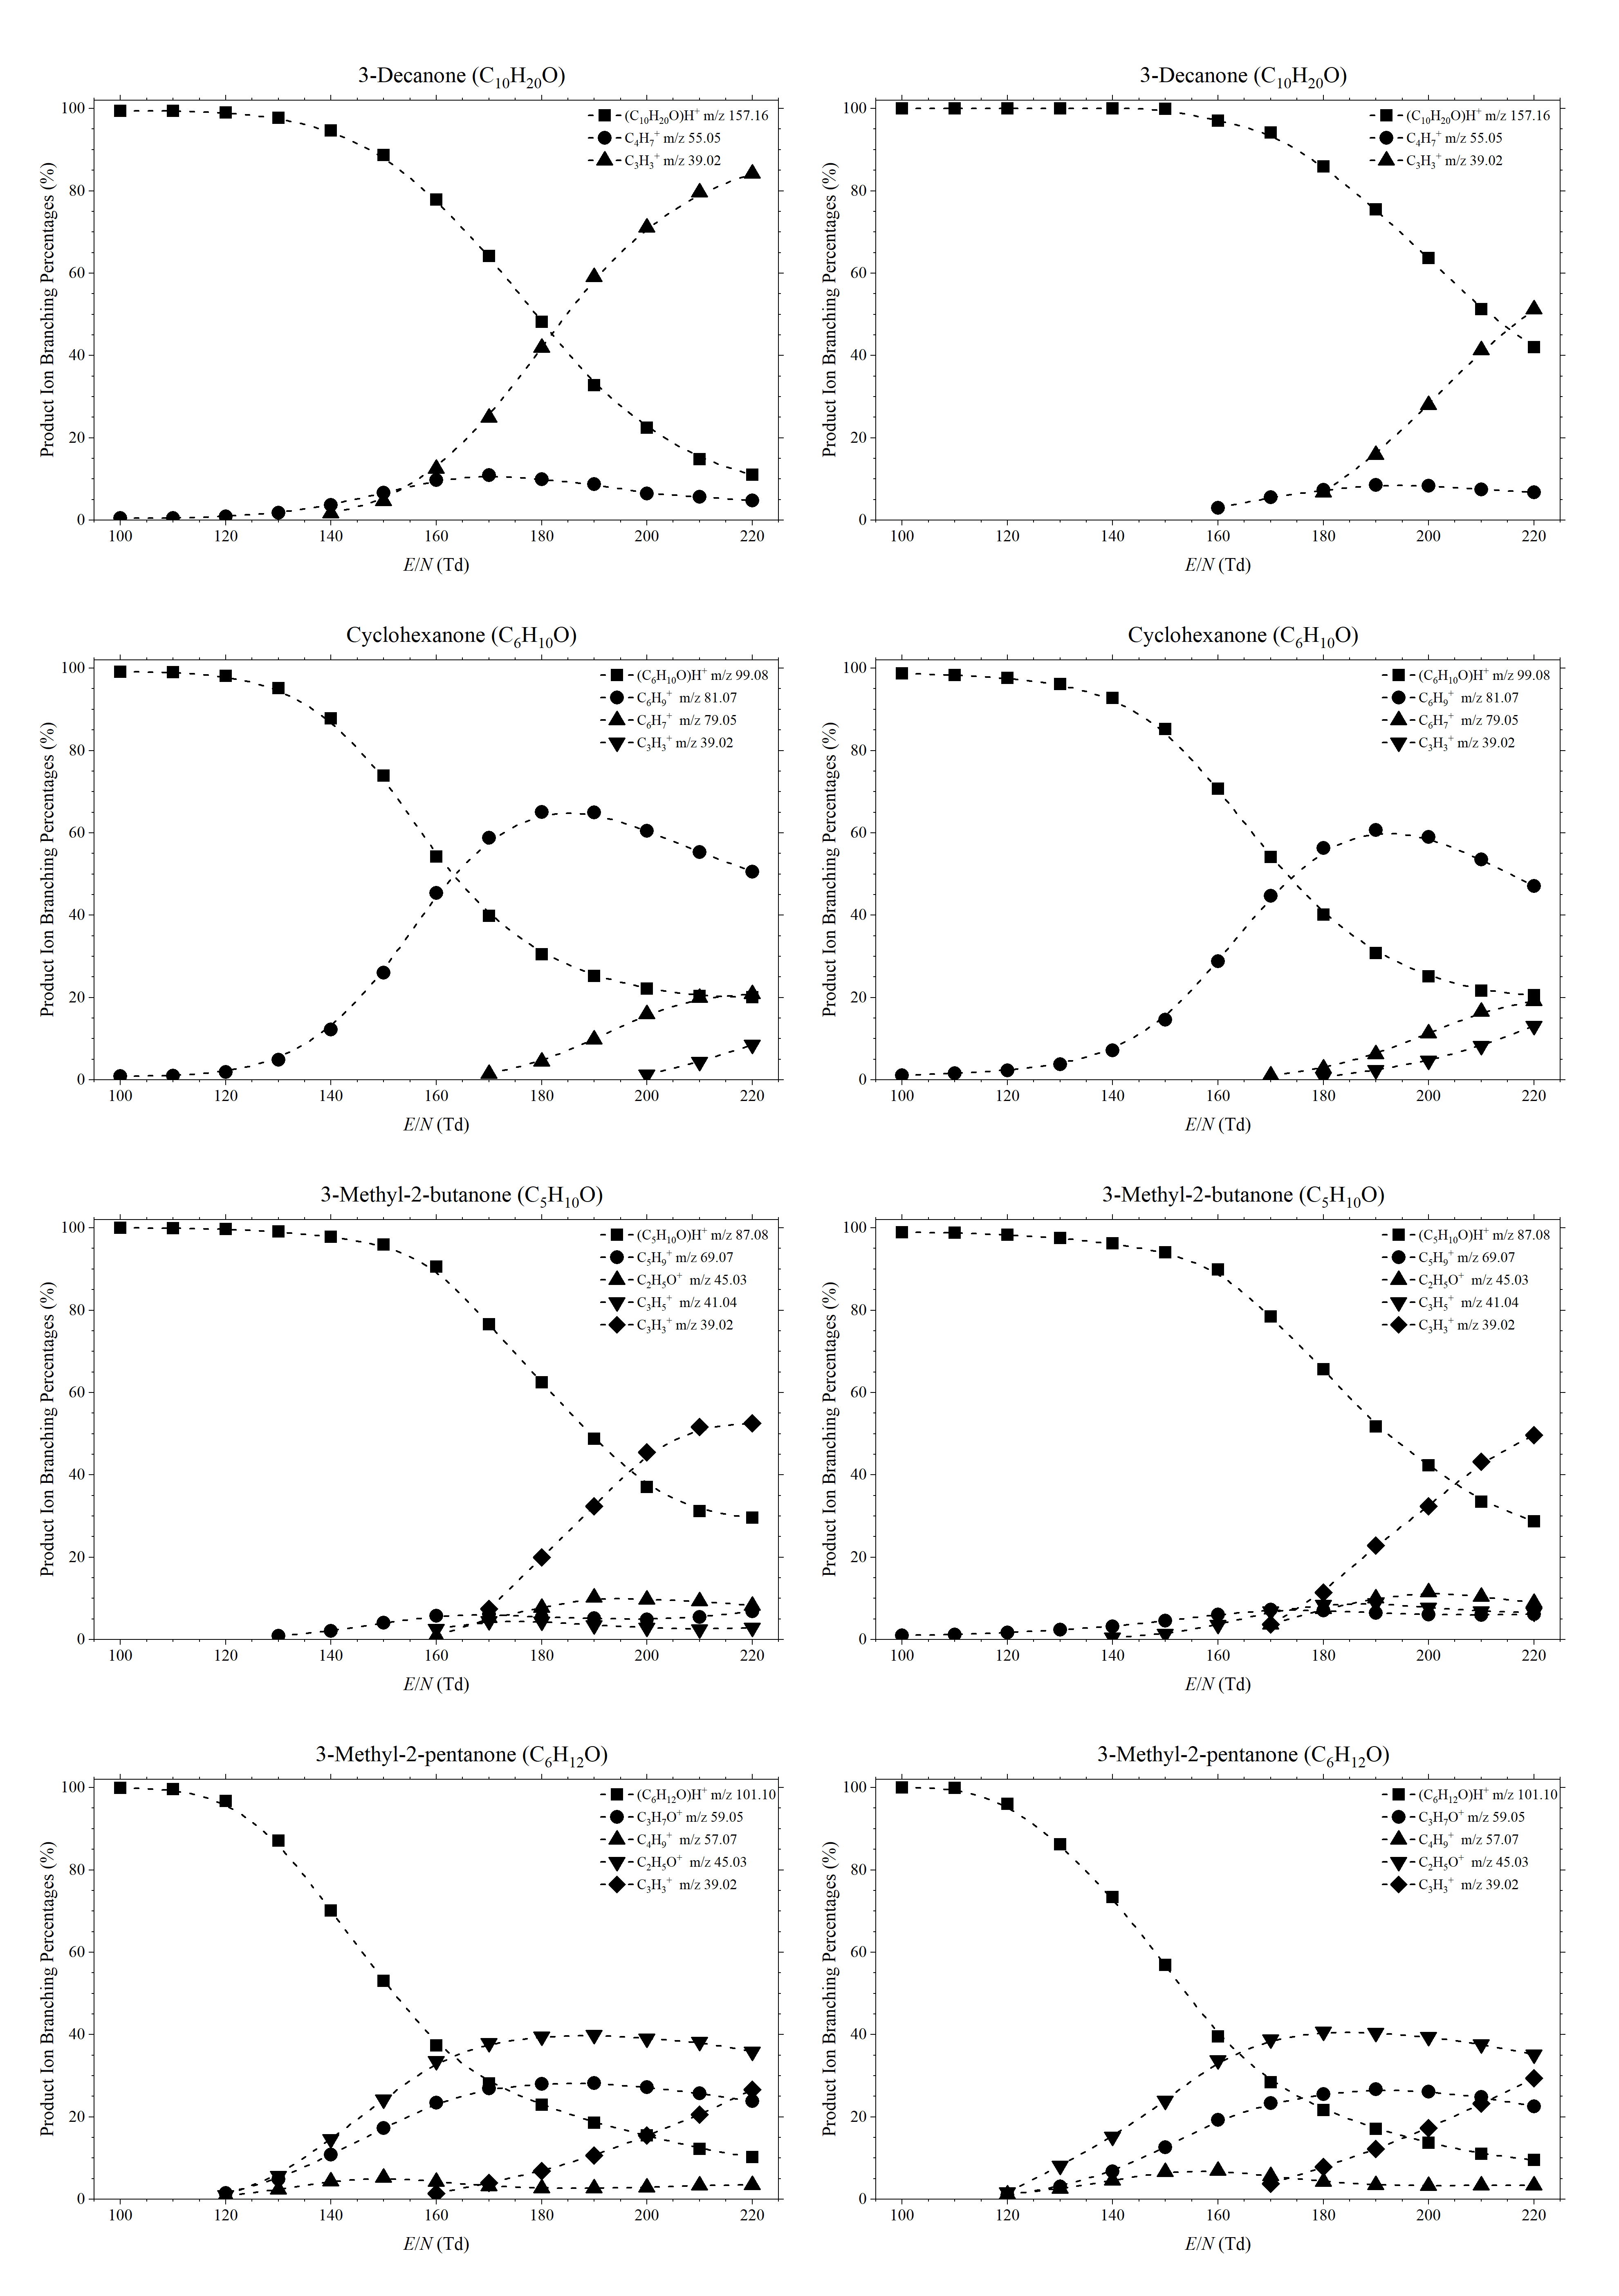
\includegraphics[width=1\textwidth]{pics/ketones/plot_5.png}
\caption{\textit{Continued}}
\end{figure}
\begin{figure}\ContinuedFloat
\centering
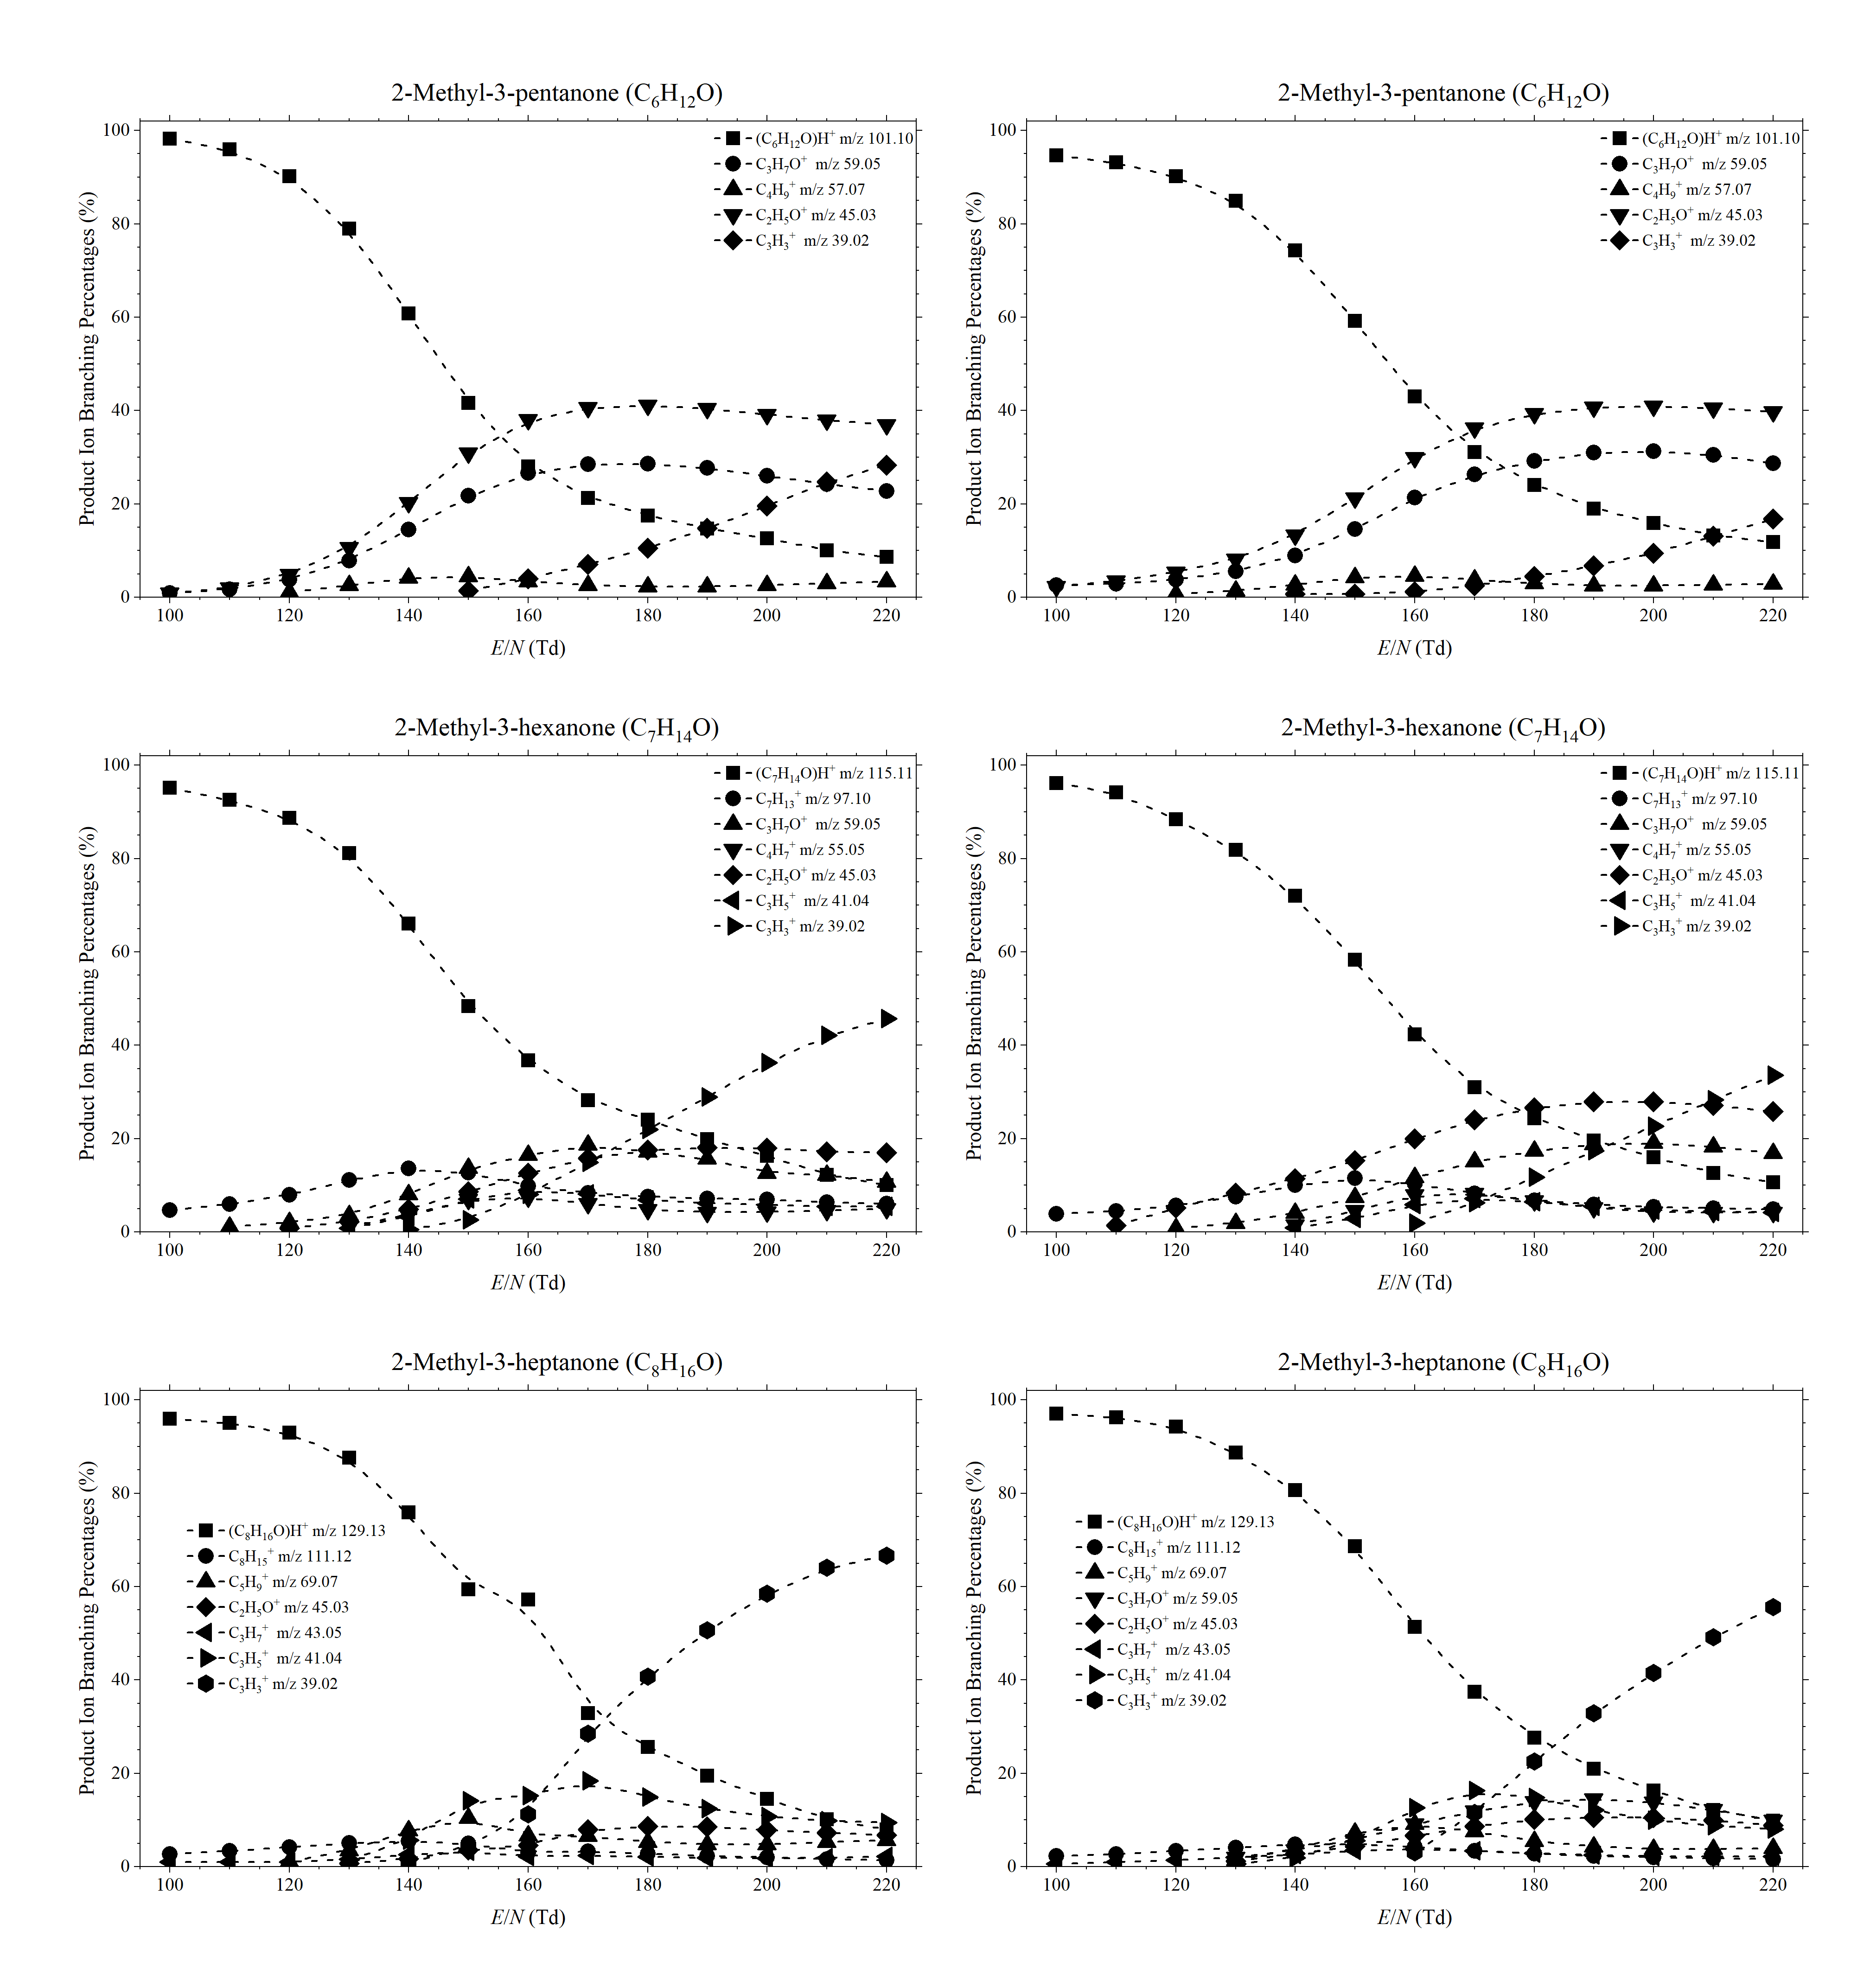
\includegraphics[width=1\textwidth]{pics/ketones/plot_6.png}
\captionsetup{list=yes}
\caption{Product ion distributions (branching percentages) as a function of \textit{E/N} resulting from reaction with H$_{3}$O$^+$ (and potentially H$_{3}$O$^+$.H$_{2}$O as stated above)
under (a) normal and (b) high humidity drift tube conditions with several ketones.}
\label{fig:ke_fig2}
\end{figure}

The protonated parent molecule is the dominant ion for all ketones at  low \textit{E/N} values (<140 Td).
This is in agreement with some studies present in the literature, like the one from \citeauthor{buhr2002analysis}, where they demonstrated that, independently of the chain length, the main reaction channel between ketones and hydronium at approximately 140 Td is non-dissociative proton transfer.
SIFT-MS \cite{vspanvel1997sift,smith2003analysis,smith2019} and SIFDT-MS \cite{spesyvyi2017ion} investigations also agree with the observation of the protonated parent being dominant at low collisional energies.

%Below approximately 140 Td, the protonated parent is the dominant product ion observed for all ketones. This is in reasonable agreement with other PTR-MS studies. For example, in the study by \citeauthor{buhr2002analysis} \cite{buhr2002analysis} at one reduced electric field of approximately 140 Td, the authors showed that proton transfer from H$_3$O$^+$ to ketones will predominantly be non-dissociative, regardless of chain length. This limited dissociation observed in PTR-MS for reduced electric fields below 140 Td also agrees with studies using the thermalized conditions in Selected Ion Flow Tube - Mass Spectrometry (SIFT-MS) \cite{vspanvel1997sift,smith2003analysis,smith2019}, and suprathermal Selected Ion Flow Drift Tube (SIFDT) investigations \cite{spesyvyi2017ion}. 


On the other hand, other product ions rather than the protonated parent molecule are observed for high \textit{E/N} values (>140 Td). This does not agree with \citeauthor{buhr2002analysis} for 2-butanone, 2-hexanone, 2-heptanone, 3-heptanone, 4-heptanone, 3-octanone, 2-nonanone and 2-decanone as they  reported the protonated parent ion as the only product ion. However, \citeauthor{buhr2002analysis} did observe for 2-pentanone, although at a lower percentage compared to our study, a product ion at \textit{m/z} 45 tentatively assigned to protonated acetaldehyde (C$_2$H$_5$O$^+$), but these discrepancies could be explained in terms of the different equipment used in each case.


%Above 140 Td, fragmentation of the protonated parent is observed, a fact that was not reported by \citeauthor{buhr2002analysis} for 2-butanone, 2-hexanone, 2-heptanone, 3-heptanone, 4-heptanone, 3-octanone, 2-nonanone and 2-decanone, for which only the protonated parent is observed. Limited fragmentation is, however, reported by \citeauthor{buhr2002analysis} at 140 Td for 2-pentanone, with a product ion being observed at \textit{m/z} 45, which we also observe and assign it to be C$_2$H$_5$O$^+$ (protonated acetaldehyde) although it is found with a much higher relative intensity compared to the protonated parent in our study than found by \citeauthor{buhr2002analysis} This difference in intensity is most probably associated with differences in the transmission of ions, because \citeauthor{buhr2002analysis} used a quadrupole mass spectrometer. 

Further discrepancies are observed when comparing our product ion distributions with those from \citeauthor{pan2017detection}, who investigated  2-butanone, 2-pentanone, 2-hexanone, 2-heptanone and cyclohexanone with a dipolar PTR-Quad-MS over over a range of low \textit{E/N} values (50-110 Td) \cite{pan2017detection}.
\citeauthor{pan2017detection} observed an unexpected amount of hydrocarbon ions (C$_n$H$_m^+$) at those collisional energies, which are also found in our investigations but only at high \textit{E/N} values. 
This is another proof showing that the findings of various PTR-MS instruments need to be compared carefully.

%In the present study, significant percentages of hydrocarbon ions, C$_n$H$_m^+$, are seen. This agrees with another \textit{E/N} study of the ketones, 2-butanone, 2-pentanone, 2-hexanone, 2-heptanone, and cyclohexanone by  \citeauthor{pan2017detection}, who used a dipolar proton transfer reaction (quadrupole) mass spectrometer \cite{pan2017detection}. Their study, which covered the reduced electric fields of approximately 50-110 Td, reported the \textit{m/z} values of the product ions we have found, but observed substantially more fragmentation than we detected, even at their low \textit{E/N} values. The amount of fragmentation reported at low \textit{E/N} (as low as 50 Td) by \citeauthor{pan2017detection} is surprising, given that at these \textit{E/N} values the reagent ion signal in our instruments would be protonated water clusters. This again illustrates that care must be taken when comparing results from different PTR-MS instruments.


In the present study, in general the protonated parent ion dominates (>80\% branching percentage) up to ca. 130 Td, although 2-7 further product ions have been observed for each ketone.
However, their contribution to the total ion signal was only noticeable at high \textit{E/N} values in most cases.
For example, of C$_3$H$_3^+$ and C$_3$H$_5^+$  only appear at reduced electric values of approximately 150 Td or higher.
The analytes showing the highest number of fragmentation channels were 3-hexanone (7 channels),
3-heptanone (6 channels),
2-methyl-3-hexanone (6 channels) 
and 2-methyl-3-heptanone (7 channels).
Higher molecular weight ketones were found to be more stable and show less  fragmentation channels.

%In our study, typically 2-7 fragmentation channels have been observed. However, many of them were significant only at higher reduced electric field values. For instance, C$_3$H$_3^+$ and C$_3$H$_5^+$ ions occur only for \textit{E/N} values higher than about 150 Td. Thus, for \textit{E/N} values up to about 130 Td, the protonated molecules are dominant having well above 80\% branching percentages associated with that channel. Interestingly, the highest number of fragmentation channels was noted for 3-hexanone (7 channels) and C7 ketones; 2-heptanone (5 channels), 3-heptanone (6 channels), 4-heptanone (5 channels) and 2-methyl-3-hexanone (6 channels). As expected, heavier ketones are found to fragment considerably less. 

Additionally, the loss of H$_2$O was also observed for some of the analysed ketones, yielding hydrocarbons with a  C$_n$H$_{2n-1}^{+}$  composition, but these represent a low percentage of the total product ion signal and also they rapidly break up at high \textit{E/N}.
Furthermore, it has been observed for C5 and C6 ketones that the fragmentation path resulting in C$_2$H$_5$O$^+$ very common.
%For several ketones, the proton transfer process is followed by the elimination of an H$_2$O molecule leading to the observed hydrocarbon ions C$_n$H$_{2n-1}^{+}$. However, these channels have small associated branching percentages, and at higher values of the reduced electric field undergo further fragmentation. 
%The channel leading to the C$_2$H$_5$O$^+$ ion is very abundant in fragmentation patterns of C5 and C6 ketones. Interestingly, the mass spectra of C8 and C9 ketones do not have oxygen-containing fragmentation channels. 

The main observed result of the higher humidity conditions is that it lessens the fragmentation of the ketones, with the product ion distributions at a given \textit{E/N} in normal conditions being comparable to those at a reduced electric field approximately 20 Td higher in humid conditions. 
This behaviour is more noticeable at mid reduced electric field values (ca. 150 Td) because of the higher presence of protonated water clusters compared to normal conditions and the emerging fragment ions at higher collisional energies.
At low \textit{E/N} the higher humidity makes no difference in this ketone study because the main observed product ion is the protonated parent. %because if the proton transfer from H$_3$O$^+$ is a non-dissociative process, so will be proton transfer from (H$_2$O)H$_3$O$^+$ as there is less energy available for fragmentation than in the former reaction (see \autoref{tb:pa}).
Also, the three body association of the protonated parent with water was not observed in any case. 
On the other side, at high \textit{E/N} the protonated water clusters are broken up through collisions with the buffer gas, which reduces this humidity effect.
This can be illustrated monitoring the protonated parent molecules from 2-pentanone and 3-nonanone, which, at 150 Td and normal and dry conditions, represent  47\% and 69\%, and 48\% and 79\%, respectively.


%High humidity reduces the fragmentation of ketones. Interestingly, this effect is most evident for the \textit{E/N} values of 150-160 Td. For example, the abundance of the protonated parent ion of 2-pentanone under normal conditions for 150 Td is 47\%; whereas, in humid air, it has a branching percentage of 69\%. The analogous values for 3-nonanone are 48\% and 79\%, respectively. This interesting dependence can be attributed to the formation of considerable amounts of protonated water clusters, which can react with ketones of interest. Consequently, far less energy is available for fragmentation in such reactions than for those associated with H$_3$O$^+$. At the higher \textit{E/N} values formation of water clusters is suppressed and, thereby, the positive effect of humidity on having reduced fragmentation is weakened. The general effect of the higher humidity is to shift the product ion branching percentage curves by approximately 20 Td to higher \textit{E/N}.



\autoref{fig:ke_fig3} presents one of the acquired mass spectra for illustrative purposes, corresponding in this case to 3-hexanone at 180 Td. This figure shows all the detected product ions, although some of them (i.e. C$_4$H$_5^+$ and C$_4$H$_9^+$) are not included in \autoref{fig:ke_fig2} or \autoref{table:ketones} because they represent less than 3\% of the total product ion signal.

%To illustrate the quality of the data, a mass spectrum recorded at 180 Td for 3-hexanone is provided in \autoref{fig:ke_fig3}. This highlights some product ions which are associated with the volatile, but are not included in the tabulation or \autoref{fig:ke_fig2}, because their contributions to the total relative abundance are less than 3\% for any reduced electric field value.



\begin{figure}%[h]
\centering
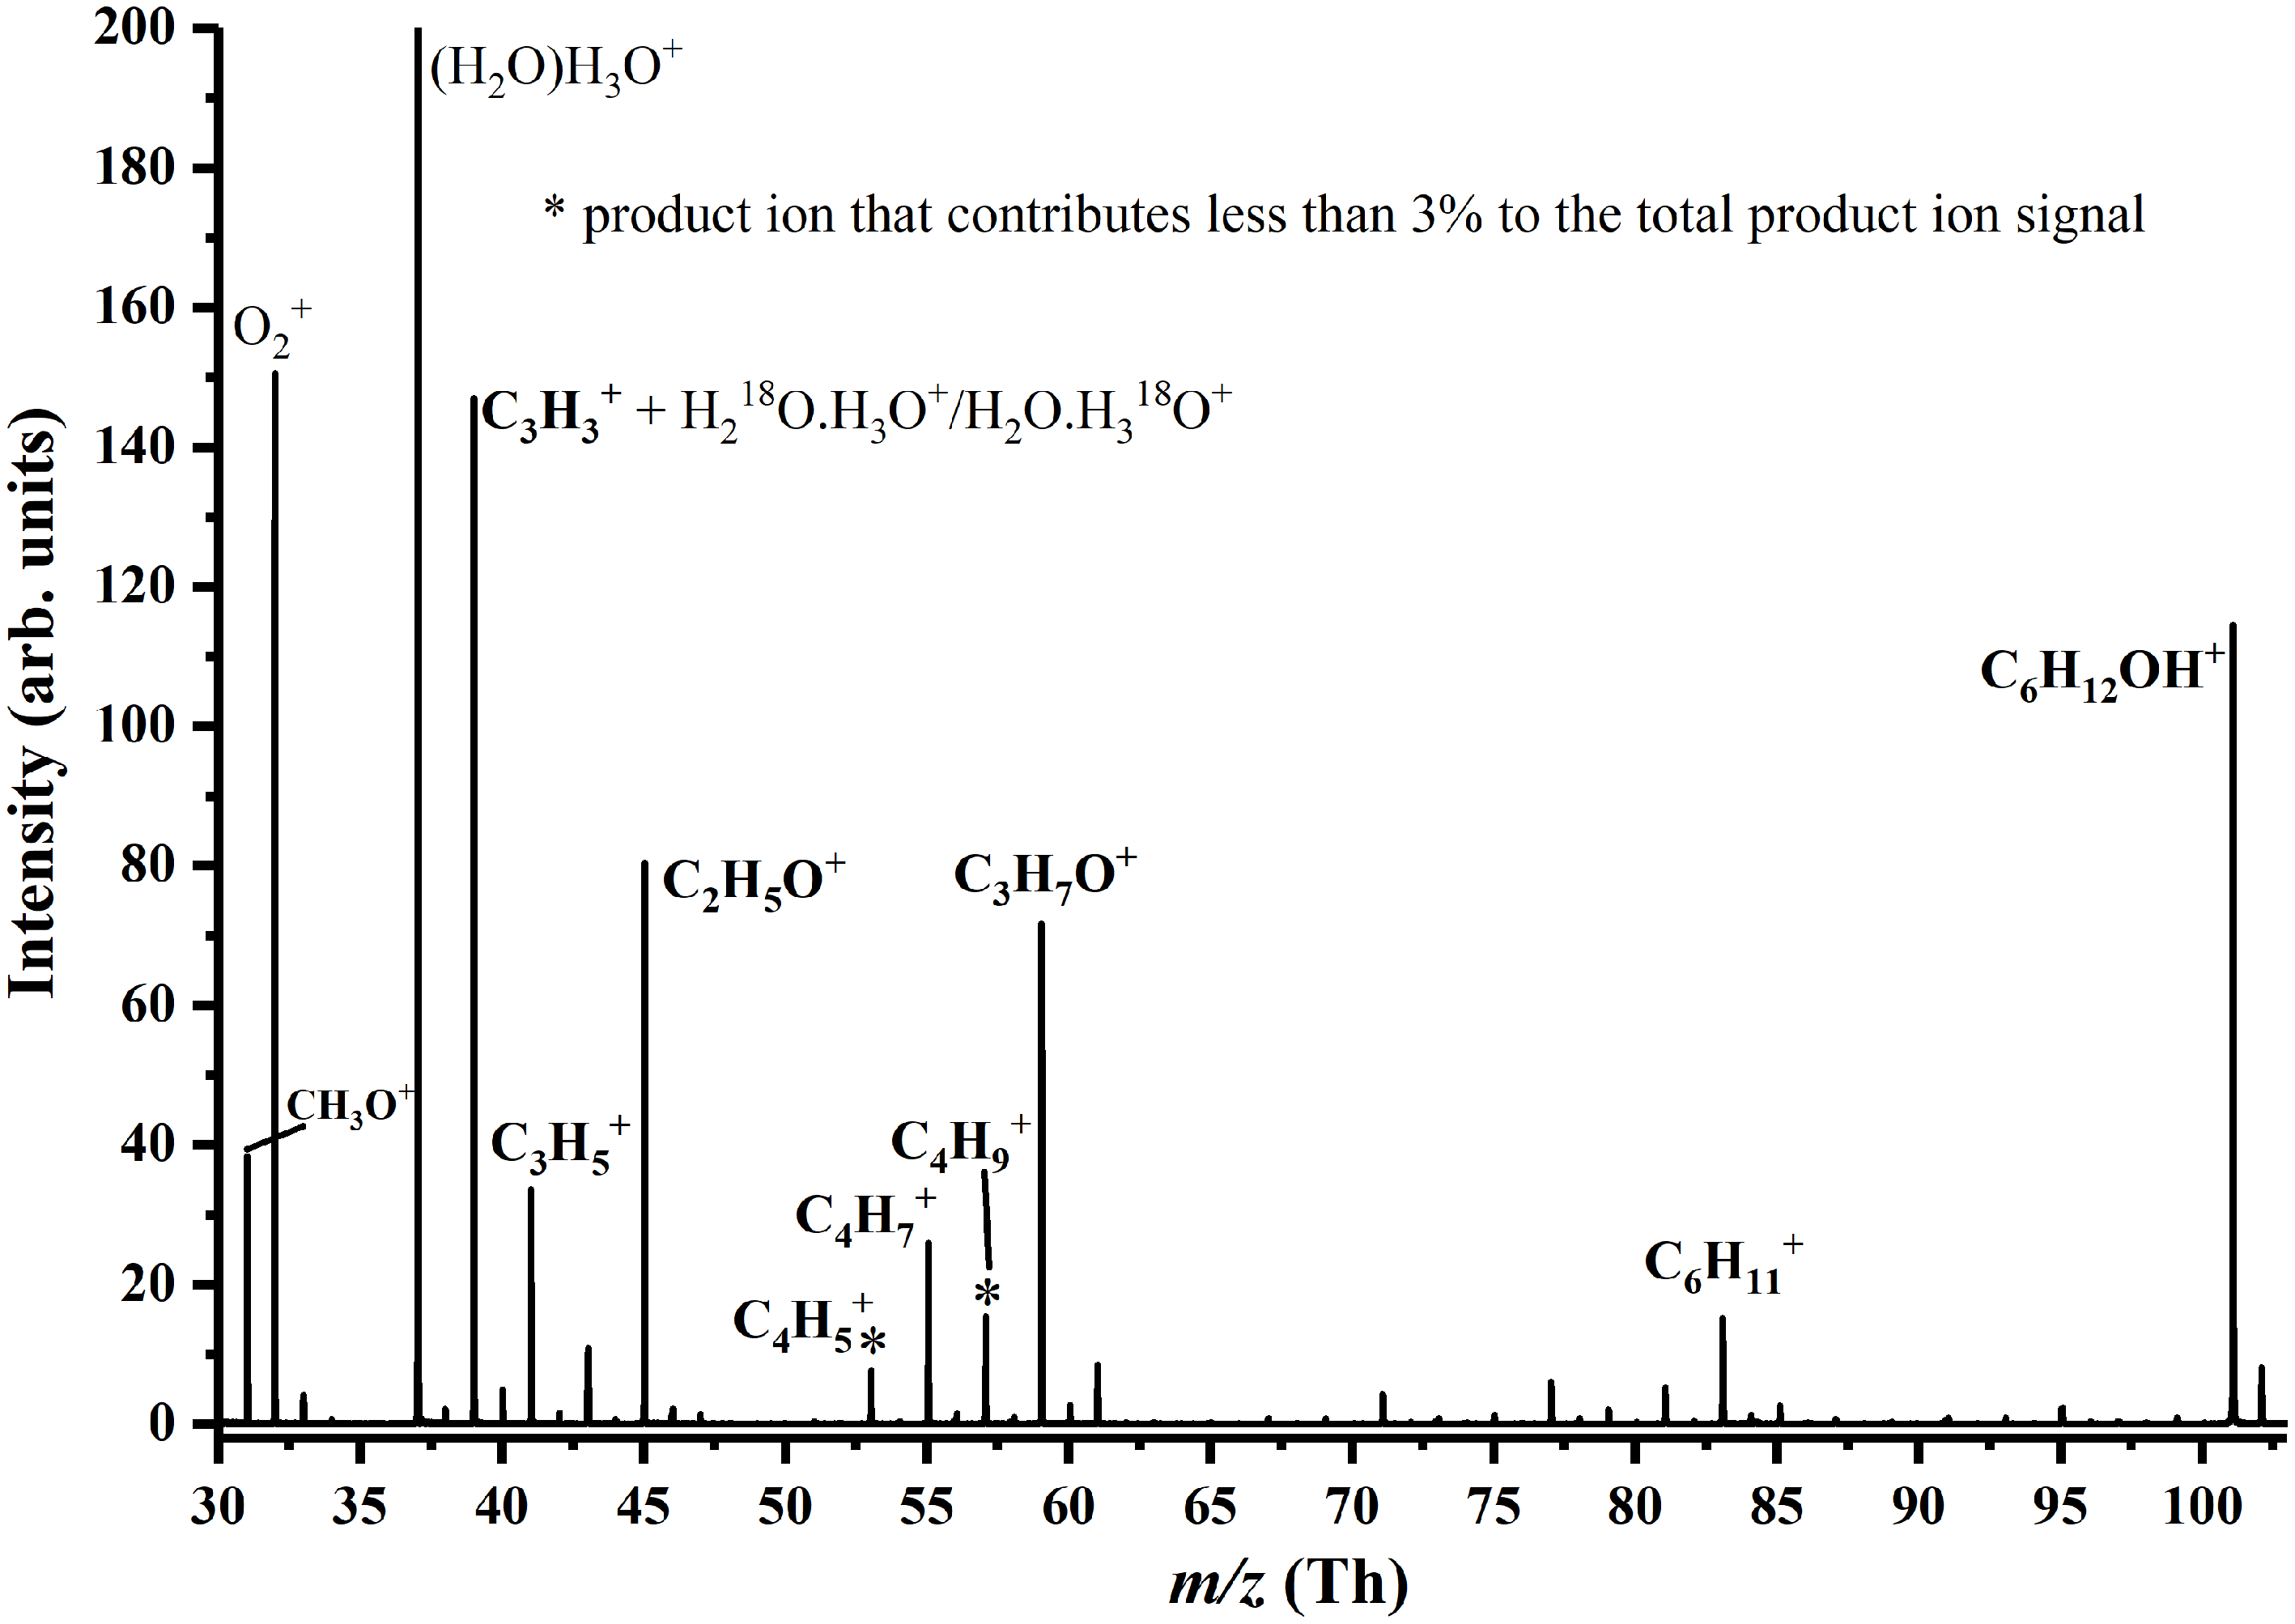
\includegraphics[height=0.35\textheight]{pics/ketones/plot_7.png}
\caption{Mass spectrum for 3-hexanone recorded at 180 Td. Product ions coming from the compound are identified. The product ions C$_4$H$_5^+$ and C$_4$H$_9^+$ each contribute <3\% to the total product ion percentage even at the highest reduced electric field investigated.}
\label{fig:ke_fig3}
\end{figure}






\section{Conclusions}
The research exposed in this chapter offers a broad database for PTR-MS users of the product ions and their relative intensities as a function of the reduced electric for the reactions of H$_3$O$^+$ and H$_3$O$^+$.(H$_2$O) with a variety of ketones.
Initially conceived thinking in the relevance of ketones in breath analysis, this study can however be relevant as well in the environmental sciences and atmospheric chemistry. 


%This work provides a large body of data and an extensive library of product ion distributions as a function of reduced electric field for the reactions of H$_3$O$^+$.(H$_2$O)$_n$ (n = 0 and 1) with a selection of ketones using the powerful analytical technique of PTR-ToF-MS. Although the study was originally conceived owing to the importance of ketones in the breath, and the need to determine what product ions should be monitored using PTR-MS, these results should be of interest to researchers working in other areas such as the environmental sciences and atmospheric chemistry. 


It is important to note that the product ion branching ratios presented here are associated to a certain PTR-MS under specific conditions (e.g humidity in the drift tube), and that these may vary when using different instrumentation and configurations. Thus, these product ion branching ratios are only indicatives of the main ion-molecule reactions and fragmentation channels occurring in the drift tube.
Also, no enhancement of selectivity was found for any of the ketones through manipulation of the collisional energy.
This means that a pre-separation stage (i.e. a fastGC device) is required when analysing ketones mixtures containing isomeric compounds (e.g. breath samples) to distinguish between them.



%A key outcome from this work is that product ion distributions at any specific reduced electric field can only be used to provide an indication of what ion-molecule channels are occurring. Detailed branching percentages are only specific to a given PTR-MS instrument and then under the specific operational conditions, not least the humidity present in the drift tube, as demonstrated in the results from this study.

%Of the ketone isomers investigated in this study, it is apparent that it is not possible to provide any selectivity by manipulating the ion chemistry through changes in the reduced electric field. For this to be accomplished, the use fast gas chromatography coupled to PTR-MS is needed when analysing gas samples that contain a mixture of ketone isomers, as often occurs in breath samples. 

A final remark is that aldehydes, which are isomers of ketones, should be accounted for when working with breath samples, as they cannot be directly separated from ketones in PTR-MS.
This needs further investigation, although one of the key differences between these two families of compounds is that aldehydes fragment remarkably more than ketones in PTR-MS, with the protonated parent ion usually representing less than 10\% of the total product ion signal \cite{buhr2002analysis,schwarz2009determining}. 
Consequently, aldehydes will only represent a small portion of the parent ions corresponding to aldehydes and ketones observed in a breath sample at low and mid reduced electric fields.







%In the context of the ketones analyses in real breath samples by PTR-MS, the functional isomers of species from this chemical family (such as e.g. aldehydes) also need to be considered and investigated as their protonated forms cannot be separated from the respective protonated ketones. The ketones’ PTR-MS analyses at the presence of their functional isomers require further studies. However, it is worth mentioning here, that aldehydes undergo significant fragmentation in the PTR-MS instruments and the abundance of their protonated parent ions is usually very small (<10\%) \cite{buhr2002analysis,schwarz2009determining}. Consequently, the presence of aldehydes in the breath sample can only have minor influence on the parent ions of the respective ketones.


%\section{Acknowledgements}
%We thank the Marie Skłodowska-Curie Actions Innovative Training Network: Ion-Molecule Processes for Analytical Chemistry Technologies (IMPACT) (www.impact-h2020itn.com) which has supported this research through the European Commission’s HORIZON 2020 Programme under Grant Agreement Number 674911. The first three authors of this paper, Michaela Malásková, David Olivenza-León and Felix Piel are Early Stage Researchers in this IMPACT network.











%\section{Introduction}
%Ketones are present in breath, faeces, urine, etc.
%They are an indicator of the metabolism...
%Reference articles humidity dependence of measurement


%\section{Methodology}
%In collaboration with IONICON Analytik GmbH (Innsbruck, Austria) and the Institute for Breath Analysis of the University of Innsbruck (Innsbruck, Austria) we measured 19 ketones, which are of interest for breath analysis. These are listed in table \ref{tb:k} and their structure is shown in figure \ref{fig:k}. We did it in dry and humid conditions and using both H$_3$O$^+$ and O$_2^+$ as reagent ions. For easier ion identification, fastGC was used when available.

%The measurements were done over different campaigns in Innsbruck, at IONICON Analytik GmbH. The data analysis was equally split between the three PhD students.

%The results have been published in a peer-reviewed journal \cite{malaskova2019compendium}.


























































%\subsection{PTR-ToF-MS 8000}
%For this study we used a PTR-ToF-MS 8000 manufactured by IONICON Analytik GmbH. This instrument has been described in detail elsewhere \cite{GRAUS20101037}. This instrument has SRI capabilities and also two add-ins were used when needed: LCU and fastGC. 




%\subsection{FastGC}
%Ask Felix information of this add-in

%\subsection{LCU}

%\subsection{Samples}



%\begin{figure}
%\begin{subfloatrow}
%\sidesubfloat[2-butanone]{\scalebox{0.7}{\begin{tikzpicture}\chemfig{[:-30]-[::60](=[::60]O)-[::-60]-[::60]}\end{tikzpicture}}
%\label{fig:k1}}
%\quad
%\sidesubfloat[]{\scalebox{0.7}{\begin{tikzpicture}\chemfig{[:-30]-[::60](=[::60]O)-[::-60]-[::60]-[::-60]}\end{tikzpicture}}
%\label{fig:k2}}
%\quad
%\sidesubfloat[]{\scalebox{0.7}{\begin{tikzpicture}\chemfig{[:30]-[::-60]-[::60](=[::60]O)-[::-60]-[::60]}\end{tikzpicture}}
%\label{fig:k3}}
%\end{subfloatrow}
%\bigskip
%\begin{subfloatrow}
%\sidesubfloat[]{\scalebox{0.7}{\begin{tikzpicture}\chemfig{[:-30]-[::60](=[::60]O)-[::-60]-[::60]-[::-60]-[::60]}\end{tikzpicture}}
%\label{fig:k4}}
%\quad
%\sidesubfloat[]{\scalebox{0.7}{\begin{tikzpicture}\chemfig{[:30]-[::-60]-[::60](=[::60]O)-[::-60]-[::60]-[::-60]}\end{tikzpicture}}
%\label{fig:k5}}
%\end{subfloatrow}
%\bigskip
%\begin{subfloatrow}
%\sidesubfloat[]{\scalebox{0.7}{\begin{tikzpicture}\chemfig{[:-30]-[::60](=[::60]O)-[::-60]-[::60]-[::-60]-[::60]-[::-60]}\end{tikzpicture}}
%\label{fig:k6}}
%\quad
%\sidesubfloat[]{\scalebox{0.7}{\begin{tikzpicture}\chemfig{[:30]-[::-60]-[::60](=[::60]O)-[::-60]-[::60]-[::-60]-[::60]}\end{tikzpicture}}
%\label{fig:k7}}
%\end{subfloatrow}
%\bigskip
%\begin{subfloatrow}
%\sidesubfloat[]{\scalebox{0.7}{\begin{tikzpicture}\chemfig{[:-30]-[::60]-[::-60]-[::60](=[::60]O)-[::-60]-[::60]-[::-60]}\end{tikzpicture}}
%\label{fig:k8}}
%\quad
%\sidesubfloat[]{\scalebox{0.7}{\begin{tikzpicture}\chemfig{[:30]-[::-60]-[::60](=[::60]O)-[::-60]-[::60]-[::-60]-[::60]-[::-60]}\end{tikzpicture}}
%\label{fig:k9}}
%\end{subfloatrow}
%\bigskip
%\begin{subfloatrow}
%\sidesubfloat[]{\scalebox{0.7}{\begin{tikzpicture}\chemfig{[:-30]-[::60](=[::60]O)-[::-60]-[::60]-[::-60]-[::60]-[::-60]-[::60]}\end{tikzpicture}}
%\label{fig:k10}}
%\quad
%\sidesubfloat[]{\scalebox{0.7}{\begin{tikzpicture}\chemfig{[:30]-[::-60]-[::60](=[::60]O)-[::-60]-[::60]-[::-60]-[::60]-[::-60]-[::60]}\end{tikzpicture}}
%\label{fig:k11}}
%\end{subfloatrow}
%\bigskip
%\begin{subfloatrow}
%\sidesubfloat[]{\scalebox{0.7}{\begin{tikzpicture}\chemfig{[:-30]-[::60](=[::60]O)-[::-60]-[::60]-[::-60]-[::60]-[::-60]-[::60]-[::-60]}\end{tikzpicture}}
%\label{fig:k12}}
%\quad
%\sidesubfloat[]{\scalebox{0.7}{\begin{tikzpicture}\chemfig{[:30]-[::-60]-[::60](=[::%60]O)-[::-60]-[::60]-[::-60]-[::60]-[::-60]-[::60]-[::-60]}\end{tikzpicture}}
%\label{fig:k13}}
%\end{subfloatrow}
%\bigskip
%\begin{subfloatrow}
%\sidesubfloat[]{\scalebox{0.7}{\begin{tikzpicture}
%\chemfig{**6(---(=[::-60]O)---)}
%\end{tikzpicture}}
%\label{fig:k14}}
%\quad\quad
%\sidesubfloat[]{\scalebox{0.7}{\begin{tikzpicture}\chemfig{[:-30]-[::60](=[::60]O)-[::-60](-[::-60])-[::60]}\end{tikzpicture}}
%\label{fig:k15}}
%\quad

%\sidesubfloat[]{\scalebox{0.7}{\begin{tikzpicture}\chemfig{[:-30]-[::60](=[::60]O)-[::-60](-[::-60])-[::60]-[::-60]}\end{tikzpicture}}
%\label{fig:k16}}
%\end{subfloatrow}
%\bigskip
%\begin{subfloatrow}
%\sidesubfloat[]{\scalebox{0.7}{\begin{tikzpicture}\chemfig{[:30]-[::-60](-[::-60])-[::60](=[::60]O)-[::-60]-[::60]}\end{tikzpicture}}
%\label{fig:k17}}
%\quad
%\sidesubfloat[]{\scalebox{0.7}{\begin{tikzpicture}\chemfig{[:30]-[::-60](-[::-60])-[::60](=[::60]O)-[::-60]-[::60]-[::-60]}\end{tikzpicture}}
%\label{fig:k18}}
%\quad
%\sidesubfloat[]{\scalebox{0.7}{\begin{tikzpicture}\chemfig{[:30]-[::-60](-[::-60])-[::60](=[::60]O)-[::-60]-[::60]-[::-60]-[::60]}\end{tikzpicture}}
%\label{fig:k19}}
%\end{subfloatrow}
%\bigskip
%\caption{Structure of (a) 2-butanone, (b) 2-pentanone, (c) 3-pentanone, (d) 2-hexanone, (e) 3-hexanone, (f) 2-heptanone, (g) 3-heptanone, (h) 4-heptanone, (i) 3-octanone,  (j) 2-nonanone, (k) 3-nonanone, (l) 2-decanone, (m) 3-decanone, (n) cyclohexanone, (o) 3-methyl-2-butanone, (p) 3-methyl-2-pentanone, (q) 2-methyl-3-pentanone, (r) 2-methyl-3-hexanone and (s) 2-methyl-3-heptanone.}
%\label{fig:k}
%\end{figure}


%\subsection{Experimental procedure}
%PTR-TOF 8000 \cite{GRAUS20101037,jordan2009online}

%FastGC \cite{romano2014wine,ruzsanyi2013multi}





%\section{Results and discussion}



%\section{Conclusions and further remarks}
%During this we (not I) found

%Shift in some humid plots, because of softened collisions due to the higher humidity

%Same study to be carried out with O$_2^+$ as reagent ion.






%\begin{table}[ht]
%\centering
%\caption{List of analysed ketones.} %(add reference, this was from PubChem).}
%\label{tb:k}
%\begin{tabular}{llcc}
%\toprule
%&\quad \textbf{Compound}	 &\textbf{Formula}\quad	&\textbf{Monoisotopic mass %(g/mol)} \quad\\ \midrule 
%\ldelim\{{13}{20mm}[\parbox{20mm}{linear}]&2-Butanone					&	%C$_{4}$H$_{8}$O		&72.107					\\
%&2-Pentanone					&	C$_{5}$H$_{10}$O	&86.134					\\
%&3-Pentanone					&	C$_{5}$H$_{10}$O	&86.134					\\
%&2-Hexanone					&	C$_{6}$H$_{12}$O	&100.161				\\
%&3-Hexanone					&	C$_{6}$H$_{12}$O	&100.161				\\
%&2-Heptanone					&	C$_{7}$H$_{14}$O	&114.188				\\
%&3-Heptanone					&	C$_{7}$H$_{14}$O	&114.188				\\
%&4-Heptanone					&	C$_{7}$H$_{14}$O	&114.188				\\
%&3-Octanone					&	C$_{8}$H$_{16}$O	&128.215				\\
%&2-Nonanone					&	C$_{9}$H$_{18}$O	&142.242				\\
%&3-Nonanone					&	C$_{9}$H$_{18}$O	&142.242				\\
%&2-Decanone					&	C$_{10}$H$_{20}$O	&156.269				\\
%&3-Decanone					&	C$_{10}$H$_{20}$O	&156.269				\\
%\addlinespace[0.1cm]
%\ldelim\{{1}{20mm}[\parbox{20mm}{cyclic}]&Cyclohexanone				&	%C$_{6}$H$_{10}$O	&98.145					\\
%\addlinespace[0.1cm]
%\ldelim\{{5}{20mm}[\parbox{20mm}{branched}]&3-Methyl-2-butanone			&	%C$_{5}$H$_{10}$O	&86.134					\\
%&3-Methyl-2-pentanone		&	C$_{6}$H$_{12}$O	&100.161				\\
%&2-Methyl-3-pentanone		&	C$_{6}$H$_{12}$O	&100.161				\\
%&2-Methyl-3-hexanone			&	C$_{7}$H$_{14}$O	&114.188				\\
%&2-Methyl-3-heptanone		&	C$_{8}$H$_{16}$O	&128.215				\\
%\bottomrule
%\end{tabular}
%\end{table}












